\documentclass[12pt]{article}
\usepackage[utf8]{inputenc} % pour le format de sortie
\usepackage[a4paper]{geometry}
\usepackage[T1]{fontenc}
\usepackage[english]{babel} % pour les accents
\usepackage{csquotes}
\usepackage{enumitem}
\usepackage{amssymb,amsmath,amsthm, amsfonts}
\usepackage{mathtools}
\usepackage{fancyhdr,multicol,accents, bbm,subcaption,caption,float,verbatim}
\usepackage[all]{xy} % for diagrams with arrows
\usepackage{tikz-cd} % for diagrams with arrows
\usepackage{graphicx} % to manage images
\usepackage{titlesec}
\usepackage{hyperref} % for hyperlinks to refs or bibliography
\usepackage{indentfirst} % for indenting the first line of a paragraph
\usepackage{optidef}
\usepackage[backend=bibtex, style=alphabetic]{biblatex} % for bibliography
\usepackage{bookmark}
\usepackage{algorithm}
\usepackage{algpseudocode}
\usepackage{chronosys}
\usepackage{csvsimple}
\usepackage{longtable}
\usepackage{caption}
\usepackage{setspace}
\addbibresource{refs.bib}

% Margins, font size =====================================================================================================================
%\oddsidemargin = 0.5cm \evensidemargin = 0.5cm \textwidth = 6.3in
%\oddsidemargin = 1.2cm \evensidemargin = 1.2cm \textwidth = 6.3in
%\textheight =8.6in
\geometry{
	a4paper,
	total={170mm,257mm},
	left=20mm,
	top=20mm,
}

% Sections (theorems, propositions, lemmas…) =====================================================================================================================
\newtheorem{theorem}{Theorem}[section]
\newtheorem{lemma}[theorem]{Lemma}
\newtheorem{corollary}[theorem]{Corollary}
\newtheorem*{conjecture}{\bf Conjecture}
\newtheorem{proposition}[theorem]{Proposition}
% \numberwithin{theorem}{section} % To display the section number in the theorem

\theoremstyle{definition}
\newtheorem{definition}[theorem]{Definition}
\newtheorem{assumption}[theorem]{Assumption}
\newtheorem{exercise}{Exercise}
\newtheorem*{solution}{Solution}
\newtheorem*{answer}{Answer}
\newtheorem*{claim}{Claim}

\theoremstyle{remark}
\newtheorem*{theoremno}{{\bf Theorem}}
\newtheorem*{remark}{Remark}
\newtheorem*{example}{Example}
\newtheorem*{hint}{Hint}



% Commands =====================================================================================================================
\def\bb#1{\mathbb{#1}}
\def\cal#1{\mathcal{#1}}
\def\frak#1{\mathfrak{#1}}
\def\rm#1{\mathrm{#1}}
\def\bf#1{\mathbf{#1}}
\newcommand{\C}{\mathbb{C}}
\newcommand{\R}{\mathbb{R}}
\newcommand{\N}{\mathbb{N}}
\newcommand{\Z}{\mathbb{Z}}
\newcommand{\Q}{\mathbb{Q}}
\newcommand{\K}{\mathbb{K}}
\newcommand{\bbP}{\mathbb{P}}
\newcommand{\F}{\mathcal{F}}
\newcommand{\calP}{\mathcal{P}}
\newcommand{\G}{\mathcal{G}}
\newcommand{\calL}{\mathcal{L}}
\newcommand{\calC}{\mathcal{C}}
\newcommand{\calN}{\mathcal{N}}
\newcommand{\calF}{\mathcal{F}}
\newcommand{\calE}{\mathcal{E}}
\newcommand{\frakA}{\mathfrak{A}}
\newcommand{\frakS}{\mathfrak{S}}
\newcommand{\esp}{\mathbb{E}}
% \P = caracs spéciaux,\S = paragraphe, \L = L barre

% Existe déjà : ker, partie Im, Re, min, max, inf, sup, log, exp, sin, sinh, cos, cosh,, tan lim, liminf, limsup
\DeclareMathOperator{\Id}{Id}
\DeclareMathOperator{\Hom}{Hom}
\DeclareMathOperator{\Ima}{Im}
\DeclareMathOperator{\Homeo}{Homeo}
\DeclareMathOperator{\Aut}{Aut}
\DeclareMathOperator{\Bij}{Bij}
\DeclareMathOperator{\Isom}{Isom}
\DeclareMathOperator{\GL}{GL}
\DeclareMathOperator{\End}{End}
\DeclareMathOperator{\rang}{rang}
\DeclareMathOperator{\rank}{rank}
\DeclareMathOperator{\vol}{vol}
\DeclareMathOperator{\sgn}{sgn}
\DeclareMathOperator{\var}{Var}
\DeclareMathOperator{\erf}{erf}
\DeclareMathOperator{\spec}{spec}
\DeclareMathOperator{\diag}{diag}
\DeclareMathOperator{\pgcd}{pgcd}
\DeclareMathOperator{\pgdc}{pgdc}

% Lois de probabilités
\DeclareMathOperator{\Geom}{Geom}
\DeclareMathOperator{\Bin}{Bin}
\DeclareMathOperator{\Exp}{Exp}
\DeclareMathOperator{\Ber}{Ber}
\DeclareMathOperator{\Student}{Student}
\DeclareMathOperator{\Poi}{Poi}
\newcommand{\czero}{\calC^0}
\newcommand{\cone}{\calC^1}
\newcommand{\ctwo}{\calC^2}
\newcommand{\cinf}{\calC^{\infty}}
\newcommand{\bigpeter}[1]{\Big\langle#1\Big\rangle}
\newcommand{\peter}[1]{\langle#1\rangle}
\newcommand{\transp}[1]{#1^t}
\newcommand{\series}[2]{\sum_{#1}^{\infty}#2}
\newcommand{\intt}[4]{\int_{#1}^{#2}#3\mathrm{d}#4}
\newcommand{\ddt}[1]{\frac{\mathrm{d}#1}{\mathrm{dt}}}
\newcommand{\deldt}[1]{\frac{\partial#1}{\partial\mathrm{t}}}
\newcommand{\rmd}[1]{\mathrm{d}#1}
\newcommand{\inv}[1]{#1^{-1}}
\newcommand{\dx}{\rmd x}
\newcommand{\dy}{\rmd y}
\newcommand{\dz}{\rmd z}
\newcommand{\dt}{\rmd t}
\newcommand{\du}{\rmd u}
\newcommand{\dv}{\rmd v}
\newcommand{\ds}{\rmd s}
\newcommand{\dxy}{\rmd xy}
\newcommand{\dyz}{\rmd yz}
\newcommand{\dyx}{\rmd yx}
\newcommand{\dzy}{\rmd zy}
\newcommand{\dzx}{\rmd zx}
\newcommand{\dxz}{\rmd xz}
\newcommand{\gtinf}[1]{\underset{#1\to\infty}{\longrightarrow}}
\newcommand{\sm}[4]{\begin{psmallmatrix}#1&#2\\#3&#4\end{psmallmatrix}}
\newcommand{\map}[4]{
	\begin{matrix}
		#1&\to&#2\\#3&\mapsto&#4
	\end{matrix}
}



\begin{document}

\begin{titlepage}
\newcommand{\HRule}{\rule{\linewidth}{0.5mm}} % Defines a new command for the horizontal lines, change thickness here

\center % Center everything on the page

%----------------------------------------------------------------------------------------
%   HEADING SECTIONS
%----------------------------------------------------------------------------------------

\vspace{3cm}
\textsc{\LARGE École polytechnique fédérale de Lausanne}\\[1.5cm] % Name of your university/college
\textsc{\Large Bachelor Project}\\[0.5cm] % Major heading such as course name
\textsc{\large Bachelor in Mathematics}\\[0.5cm] % Minor heading such as course title

%----------------------------------------------------------------------------------------
%   TITLE SECTION
%----------------------------------------------------------------------------------------

\begin{doublespace}
    \HRule \\[0.4cm]
    \huge \bfseries Study of Relaxed Recentered Log-Barrier function based Nonlinear Model Predictive Control\\[0.4cm]
    \HRule \\[1.5cm]
\end{doublespace}

%----------------------------------------------------------------------------------------
%   AUTHOR SECTION
%----------------------------------------------------------------------------------------

\begin{minipage}{0.4\textwidth}
\begin{flushleft} \large
\emph{Author:}\\
Tudor \textsc{Oancea} % Your name
\end{flushleft}
\end{minipage}
~
\begin{minipage}{0.4\textwidth}
\begin{flushright} \large
\emph{Supervisors:} \\
Nicolas \textsc{Boumal}\\
Colin \textsc{Jones}
\end{flushright}
\end{minipage}

\vfill % Fill the rest of the page with whitespace

%----------------------------------------------------------------------------------------
%   LOGO SECTION
%----------------------------------------------------------------------------------------


\includegraphics[width=0.4\linewidth]{Logo}\\[1cm] % Include a department/university logo - this will require the graphicx package

%----------------------------------------------------------------------------------------


\end{titlepage}


\clearpage
\thispagestyle{empty}
\begin{abstract}
	In this project, we investigate the use of relaxed recentered logarithmic barrier functions in the context of Nonlinear Model Predictive Control (Nonlinear MPC or NMPC).
	These functions are a variation of the regular log-barrier functions that are introduced in the objective function of an optimization problem as a penalty on the deviation from the constraints set.
	The resulting new MPC scheme has been studied in the case of linear dynamics, and several interesting results on the global nominal asymptotic stability of the corresponding closed-loop system and on constraint satisfaction guarantees have been obtained.
	Extending them to the case of nonlinear dynamics is a non trivial task and we show in this project that these properties can still hold, but only locally.
	The theoretical results are complemented by numerical illustrations based on the Real Time Iteration method.
\end{abstract}

\clearpage
\thispagestyle{empty}
\tableofcontents

\clearpage
\pagenumbering{arabic}
\setcounter{page}{1}


\section{Introduction}
\textit{Control theory} can simply be defined as the study of a dynamical system whose state evolution can be influenced by the means of external parameters called \textit{controls}, or \textit{inputs}.
This theory is of major importance in numerous fields of engineering such as robotics, mechanical or chemical engineering where problems such as stabilizing a chemical reaction at a certain temperature or making an autonomous car follow the road are common.

An important subfield of control theory is \textit{optimal control}, which attempts to find a \textit{control law}, i.e. a policy used to control a system in order to accomplish a certain goal, by formulating and solving an optimization problem.
For example, if one wants to stabilize the state around a reference point that is constant in time, one will want to choose a control law that will minimize the distance between the future state (that depends on the current state and the chosen control) and the target state.
This problem of \textit{stabilization} will be the one we will consider in this paper, but it is interesting to know there are other problems for which optimal control is applicable, such as path tracking or optimal trajectory generation.

One of the most important algorithm of optimal control is \textit{Model Predictive Control}, or MPC.
This procedure uses the knowledge of the system's \textit{model} (the equation governing its evolution) to compute a control law that also takes the future into account.
More precisely, the control law is computed for an interval in time called the \textit{horizon}, and the cost along this whole horizon is minimized.
In some sense, the controller tries not to take decisions it will regret afterwards.
MPC has many advantages over other classical control strategies, such as the ability to handle several control parameters and to take into consideration constraints on the states and the controls (by solving a \textit{constrained} optimization problem).
These are very important in practice because any real-life system has physical limitations (e.g. the maximum speed of a car, the maximum torque of a motor, etc.).
We will properly introduce the mathematical formulation of MPC and the theoretical tools used to study it in section~\ref{sec:background-material}.

In section~\ref{sec:RRLB-MPC} we will introduce a different formulation in which (most of) the state and control constraints are replaced with a penalty added to the cost function in the form of a log-barrier function, which are common in Interior Point methods.
These functions have several drawbacks, such as the fact that they are only defined in the interior of the feasible set.
In this paper we will introduce a relaxed version of these functions called \textit{Relaxed Recentered Log-Barrier functions}, or \textit{RRLB functions}.
They extend regular log-barrier functions to the whole space and yield an equality-only-constrained optimization problem, which should in general be easier to solve.
% More details on the upsides of RRLB functions can be found in the Introduction of \cite{RRLB-linear-MPC}.

In the theoretical study of this new formulation that we will call \textit{RRLB MPC}, we will prove two major results:

\begin{enumerate}
	\item When using the control law computed by the RRLB MPC, the corresponding closed-loop system asymptotically stabilizes at the target state (see subsection~\ref{sec:RRLB-nominal-stability}).
	This property will be called \textit{nominal stability}, to be differentiated of \textit{real-time stability} (see subsection~\ref{sec:RRLB-real-time-stability}).
	\item In this formulation, the optimal solution of the optimization problem might yield states or controls that are not feasible in the original problem, since the constraints are not strictly enforced.
	However, if we start sufficiently close to the target state, this will never happen (see subsection~\ref{sec:constraints-satisfaction-guarantees}).
\end{enumerate}

Finally, in section~\ref{sec:RRLB-numerical-aspects} we examine numerical aspects of the RRLB MPC.
We will introduce a common strategy to solve NMPC problems called \textit{Real Time Iteration} (or RTI) and discuss its advantages and drawbacks as for the tradeoff between computational efficiency and accuracy.
A simple Python implementation of this method will be used to verify our theoretical results and to compare the performance of RRLB MPC and regular MPC (eg in terms of runtime and in terms of convergence speed).
The system of choice will be a popular benchmark problem called \textit{Continuously Stirred Tank Reactor} (or CSTR).

\section{Background material}\label{sec:background-material}

This whole section constitutes classical knowledge on MPC and dynamical system and can references can be found in textbooks such as \cite{MPC-book} (chapters 1 and 2 on MPC and Appendix B on stability theory) or \cite{MPC-book-2} (chapter 3 on NMPC and chapter 4 on infinite horizon MPC).

\subsection{What is MPC ?}\label{sec:what-is-MPC}

We consider a discrete-time controlled nonlinear dynamical system of the form $x(k+1)=f(x(k), u(k))$ (which we will usually write as $x^+=f(x,u)$) with state and control constraints $x(k)\in\cal{X}\subseteq\R^{n_x},~u(k)\in\cal{U}\subseteq\R^{n_u}$.

In practice, the systems of interest are almost always continuous. We therefore assume that we will only change the control variables at instants evenly spaced in time, and we discretize the dynamics using ODE integrators such as RK4. The time between each two consecutive control updates is called the \textit{sampling time}.

Our goal is to stabilize the system around a target state $x^*$ and a target control $u^*$, which have to be a fixed point of the system: $x^*=f(x^*, u^*)$\,.
To do that we will try to construct a \textit{state-feedback control law}, i.e. a function $\mu:\cal{X}\to\cal{U}$ such that $x^*$ is \textit{asymptotically stable} for the dynamical system $x^+=f(x,\mu(x))$ (which only depends on the state).
The exact definition of asymptotical stability and how to prove it is discussed in subsection~\ref{sec:Lyapunov-stability-theory}.

An important simplification that is often made (and that we will use in this paper) is that we consider $x^*=0$ and $u^*=0$\,.
It is easy to verify that when this is not the case, we can just define new translated states $\hat{x}=x-x^*$ and new control $\hat{u}=u-u^*$ and consequently new dynamics, new constraints, etc.

\noindent To construct this control law $\mu$, we will solve the following optimization problem:

\begin{align}
	\begin{split}
		\label{eq:NMPC}
		V_N(x)=\underset{\bf{x},\bf{u}}{\min} &\quad \sum_{k=0}^{N-1}l(x_k,u_k)~+~F(x_N)\\
		\text{s.t.} &\quad x_0=x\text{ and }x_{k+1}=f(x_k,u_k),~k=0,\ldots,N-1\\
		&\quad x_k\in\cal{X},~k=0,\ldots,N\\
		&\quad u_k\in\cal{U},~k=0,\ldots,N-1
	\end{split}
\end{align}

\noindent where $N\in\N$ is called the \textit{horizon length}, the function $l:\cal{X}\times\cal{U}\to\R$ is the \textit{stage cost}, the function $F:\cal{X}\to\R$ is the \textit{terminal cost} (its role will become clearer in next section) and the function $J_N:\cal{X}^{N+1}\times\cal{U}^N\to\R, (\bf{x},\bf{u})\mapsto\sum_{k=0}^{N-1}l(x_k,u_k)~+~F(x_N)$ is called the \textit{cost function}.

\vspace{12pt}

These costs have to be defined by the user as a measure of the deviations from the target state and control (we will always assume that $l(x^*,u^*)=l(0,0)=0$).
Their fine tuning is of capital importance for the feasibility, robustness and performance of the MPC scheme, and it is a whole area of interest of control theory (which is unfortunately out of the scope of this paper).
Then, during the experiment, we observe at a time $k$ the state $x(k)$, we solve the MPC~\ref{eq:NMPC} and find the optimal sequences of states and controls $$\bf{x}^*(x(k))=\left\{ x_0^*(x(k))=x(k),\ldots,x_N^*(x(k))\right\},\quad \bf{u}^*(x(k))=\left\{ u_0^*(x(k)),\ldots,u_{N-1}^*(x(k))\right\}$$
They represent the controls to apply at time $k,k+1,\ldots,k+N-1$ and the states the system will be in after these controls are applied.
In a sense, we 'over-solve' the problem since we are actually only interested in $u_0^*(x(k))$ that will define our control law:
$$\mu_{\rm{MPC}}(x(k)):=u_0^*(x(k))$$
Since at time $k+1$ the horizon will have shifted, we say we solve the control problem in a \textit{receding horizon} fashion.

\vspace{12pt}

Other variants of MPC exist in which different state constraint, called \textit{terminal constraints}, are enforced on $x_N$\,.
We are also going to consider very specific forms of costs and constraints: the costs will always be quadratic ($l(x,u)=x^TQx+u^TRu$ and $F(x)=x^TPx$ for some symmetric and positive definite matrices $Q,R$ and $P$) and the (inequality) constraints will always be polytopic (of the form $\cal{X}=\left\{x\in\R^{n_x}~|~C_xx\leq d_x\right\},~\cal{U}=\left\{u\in\R^{n_u}~|~C_uu\leq d_u\right\}$ for matrices $C_x,C_u$ and vectors $d_x,d_u$ of appropriate dimension such that the sets are bounded).
These are very common in real-world applications.

\vspace{12pt}

\noindent Other variants of MPC are:
\begin{itemize}[label=\textbullet]
	\item \underline{the \textit{infinite horizon MPC}}:
	\begin{align*}
		V_\infty(x)=\underset{\bf{x},\bf{u}}{\min} &\quad \sum_{k=0}^{\infty}l(x_k,u_k)\\
		\text{s.t.} &\quad x_0=x\text{ and }x_{k+1}=f(x_k,u_k),~k=0,\ldots,N-1\\
		&\quad x_k\in\cal{X},~k=0,\ldots,N\\
		&\quad u_k\in\cal{U},~k=0,\ldots,N-1
	\end{align*}
	In real life applications, we consider that the duration of the experiment is virtually infinite, so this variant may seem more natural.
	It is usually not used in practice as the optimization problem becomes infinite-dimensional, which is in general computationally intractable.

	However, it enjoys several theoretical properties such as \textit{Bellman's principle of optimality}(see \cite{Bellman:DynamicProgramming}) that can be defined in the following way:
	\begin{quotation}
		\textit{An optimal policy has the property that whatever the initial state and initial decision are, the remaining decisions must constitute an optimal policy with regard to the state resulting from the first decision.}
	\end{quotation}
	or in mathematical terms:

	\begin{equation}
		\label{eq:inf-bellman}
		V_\infty(x)=l(x,u_0^*(x))+V_\infty(x,f(x,u_0^*(x)))=\min_{u\in\cal{U}}~l(x,u)+V_\infty(x,f(x,u))
	\end{equation}

	\noindent This recursive minimization problem forms the basis of what we call \textit{Dynamic Programming}, and relies on the fact that the horizon is infinite.
	In the finite horizon case (without terminal costs) a weaker version reads:

	$$V_N(x)=\min_{u\in\cal{U}}~l(x,u)+V_{N-1}(x,f(x,u))$$

	The terminal costs in regular MPC can actually be interpreted as a proxy for the part of the infinite horizon that is not considered and are present to bridge the gap between finite horizon performance and infinite horizon optimality.
	As it is illustrated in the next point, in some cases $V_\infty$ can actually be computed exactly.


	\item\underline{the \textit{(infinite-horizon) Linear Quadratic Regulator}, or \textit{LQR}}:\newline
	which is basically an MPC with linear dynamics ($x^+=Ax+Bu$) and without state and control constraints.
	These problem is the most basic one we can find and is deeply linked to the  \textit{(Discrete) Algebraic Riccati Equations}, or \textit{DARE}:
	\begin{equation}
		\label{eq:DARE-LQR}
		P=Q+A^TPA-A^TPB(R+B^TPB)^{-1}B^TPA
	\end{equation}
	This equation derived from the Bellman's principle of optimality evoked above allows us to solve the dynamic programming problem~\ref{eq:inf-bellman} explicitly: the unique positive definite solution $P$ of this equation verifies $V_\infty(x)=x^TPx$.
	The proof of the existence of this unique solution belongs to the classical control theory, is not strictly necessary to understand this project and is therefore omitted.


	The DARE theory also provides the state-feedback control law of the infinite horizon LQR: $\mu_{\rm{LQR}}(x)=Kx$ where $K=-(R+B^TPB)^{-1}B^TPA$\,.
	It is interesting to notice that in this case, the solution $P$ to the DARE also verifies the following equation called \textit{Lyapunov equation}:
	$$P=A_K^TPA_K+Q_K$$
	where $A_K:=A+BK$ corresponds the evolution of the controlled system since $x^+=Ax+B\mu(x)=(A+BK)x$, and $Q_K:=Q+K^TRK$ corresponds to cost of a stage $(x,Kx)$ since $l(x,Kx)=x^TQ+(Kx)^TR(Kx)=x^TQ_Kx$\,.

	All the derivation of the previous facts can be found in the appendix~\ref{sec:DARE}.
	In most cases, the terminal costs of a finite horizon MPC are constructed by solving a variation of the DARE that stems from a LQR approximating the original M¨PC.
\end{itemize}


\subsection{Lyapunov stability theory}\label{sec:Lyapunov-stability-theory}
In this subsection we present the necessary background in dynamical systems theory and in particular give more precise definitions of the stability properties we want to prove.
We will consider a general nonlinear dynamical system $x^+=g(x)$, without any control, since we remember that our goal is to construct the control as only depending on the state.

\noindent A state $x^*$ is said to be:
\begin{itemize}[label=\textbullet]
	\item \textit{locally stable} if $\forall\epsilon>0,\exists \delta>0$ s.t. $\|x(0)-x^*\|\leq\delta\implies\|x(k)-x^*\|\leq\epsilon,~\forall k\geq 0$\, or in other words if when the system starts close to $x^*$, it always stays close to it.
	\item \textit{locally attractive} if $\|x(k)-x^*\|\underset{k\to\infty}{\longrightarrow}0$ for all $x(0)$ in a neighborhood of $x^*$\, or in other words if when the system starts close to $x^*$, it will converge to it.
	\item \textit{globally attractive} if $\|x(k)-x^*\|\underset{k\to\infty}{\longrightarrow}0$ for all $x(0)\in\cal{X}$\, or in other words that the system will converge to it no matter the initial state.
	\item \textit{locally asymptotically stable}, or \textit{LAS}, if it is both locally stable and locally attractive.
	\item \textit{globally asymptotically stable}, or \textit{GAS}, if it is both stable and globally attractive.
\end{itemize}

It can be showed that a state $x^*$ is GAS (respectively LAS), if we can find a function $V:\cal{X}\to\R$ and constants $c_1,c_2,c_3>0$ such that $\forall x\in\cal{X}$ (respectively in a neighborhood of $x^*$):
\begin{align*}
	V(x)&\leq c_1\|x-x^*\|^2\\
	V(x)&\geq c_2\|x-x^*\|^2\\
	V(g(x))&\leq V(x)-c_3\|x-x^*\|^2
\end{align*}
Such a function is called a \textit{Lyapunov function}, and the last equation is called the \textit{descent property}, which is usually the one that is the harder to prove for a given candidate function.

\vspace{12pt}

When considering a system controlled by MPC as described in section~\ref{sec:what-is-MPC}, the candidate function of choice will be the objective value function $V_N$ defined in~\ref{eq:NMPC}.
General conditions that ensure this property can be found in chapter 2 section 4 of \cite{MPC-book}.



\section{The RRLB MPC}\label{sec:RRLB-MPC}

In this section we will introduce the RRLB functions, formulate the RRLB MPC and recall the results proved in the linear case in \cite{RRLB-linear-MPC}.
As mentioned in the last section, we will suppose that $x^*=0\in\cal{X}^\circ$ and $u^*=0\in\cal{U}^\circ$.

Before introducing the RRLB MPC, let's first state the principal problem it solves.
In practice, it might happen than the constraints are violated because of external disturbances or of the presence of \textit{model mismatch}, i.e. the system's evolution is not perfectly described by the dynamics used in the MPC.
In this case, the NLP defining the MPC~\ref{eq:NMPC} becomes unfeasible and the algorithm implementing it will either crash or return solutions that are not optimal at all.
A common way to fix this problem was to use soft constraints on the state and control constraints, by introducing slack parameters that are penalized in the objective function.
Such approaches were reported for example in \cite{soft-constrained-MPC}.
The problem with this soft-constrained formulation is the incapacity of providing closed-loop properties like asymptotic stability or constraints satisfaction, unless nonsmooth penalty functions are used, which dramatically impacts the algorithms in charge of solving the NLP.
RRLB functions are designed to overcome this limitations while still preserving the recursive feasibility properties.

\vspace{12pt}

Let's first take a step back and recall what regular log-barrier functions are.
We will only give the definitions for the states $x\in\R^{n_x}$, since they only depend on the constraint set and not on the actual quantity represented.

For a simple constraint of the form $c^Tx\leq d$, the associated \textit{log-barrier function} is defined as $-\log(d-c^Tx)$.
Such a function is defined on the interior of feasible set of the constraint and becomes infinity near its boundary.
For a set of polytopic constraints $\left\{ x~|~C_xx\leq d_x \right\}$, we can define the log-barrier as the sum of the log-barriers for each constraint:
$$B_x(x)=\sum_{i=1}^{q_x}-\log(d_{x,i}-\rm{row}_i(C_x)x)$$
where $q_x$ is the number of constraints, or equivalently the numbers of rows in $C_x$\,.

A first interesting property we would like to add to our log-barrier function is the one of \textit{positive definiteness}, i.e. $B_x(x)>0,~\forall x\neq 0$ in a neighborhood of the origin.
To this end we introduce the notion of \textit{weight recentered log-barrier function} as defined in \cite{RLB}:
$$B_x(x)=\sum_{i=1}^{q_x}(1+w_{x,i})\left[\log(d_{x,i})-\log(d_{x,i}-\rm{row}_i(C_x)x)\right]$$
where the weights $w_{x,i}$ are defined as chosen such that $B_x(0)=0$ and $\nabla B_x(0)=0$.
It is shown in \cite{RLB} that such weights always exist when the constraint set is polytopic (i.e. polyhedral and bounded) and that this wight-recentered log-barrier function is also positive definite and upper-bounded by a quadratic.

The second important property we have to add is the definiteness on the whole space.
For a given \textit{relaxation parameter} $\delta>0$, we can define the \textit{relaxed recentered log-barrier function}, or \textit{RRLB} function as follows:
\begin{align}
	\begin{split}
		\label{RRLB}
		B_x(x)&=\sum_{i=1}^{q_x}(1+w_{x,i})B_{x,i}(x)\\
		\text{ with }B_{x,i}(x)&=\begin{cases}
			\log(d_{x,i})-\log(d_{x,i}-\rm{row}_i(C_x)x)&\text{if }d_{x,i}-\rm{row}_i(C_x)x>\delta\\
			\beta(d_{x,i}-\rm{row}_i(C_x)x;\delta)&\text{ otherwise}
		\end{cases}
	\end{split}
\end{align}
where $\beta$ is a twice continuously function that extends the log-barrier to a twice continuously differentiable function on $\R$.
The simplest example of such a function is
$$\beta(z;\delta)=\frac{1}{2}\left[ \left( \frac{z-2\delta}{\delta} \right)^2-1 \right]-\log(\delta)$$
To ensure that this function still verifies $B_x(0)=0$ and $\nabla B_x(0)=0$, we need to choose $0<\delta\leq\min\left\{d_{x,1},\ldots,d_{x,q_x},d_{u,1},\ldots,d_{u,q_u}\right\}$\,, which is always possible if $0\in\cal{X}$ and $0\in\cal{U}$\,.
An illustration of this relaxation procedure can be found in figure~\ref{fig:RRLB-functions} found in \cite{rti-diehl}.

\begin{figure}
	\centering
	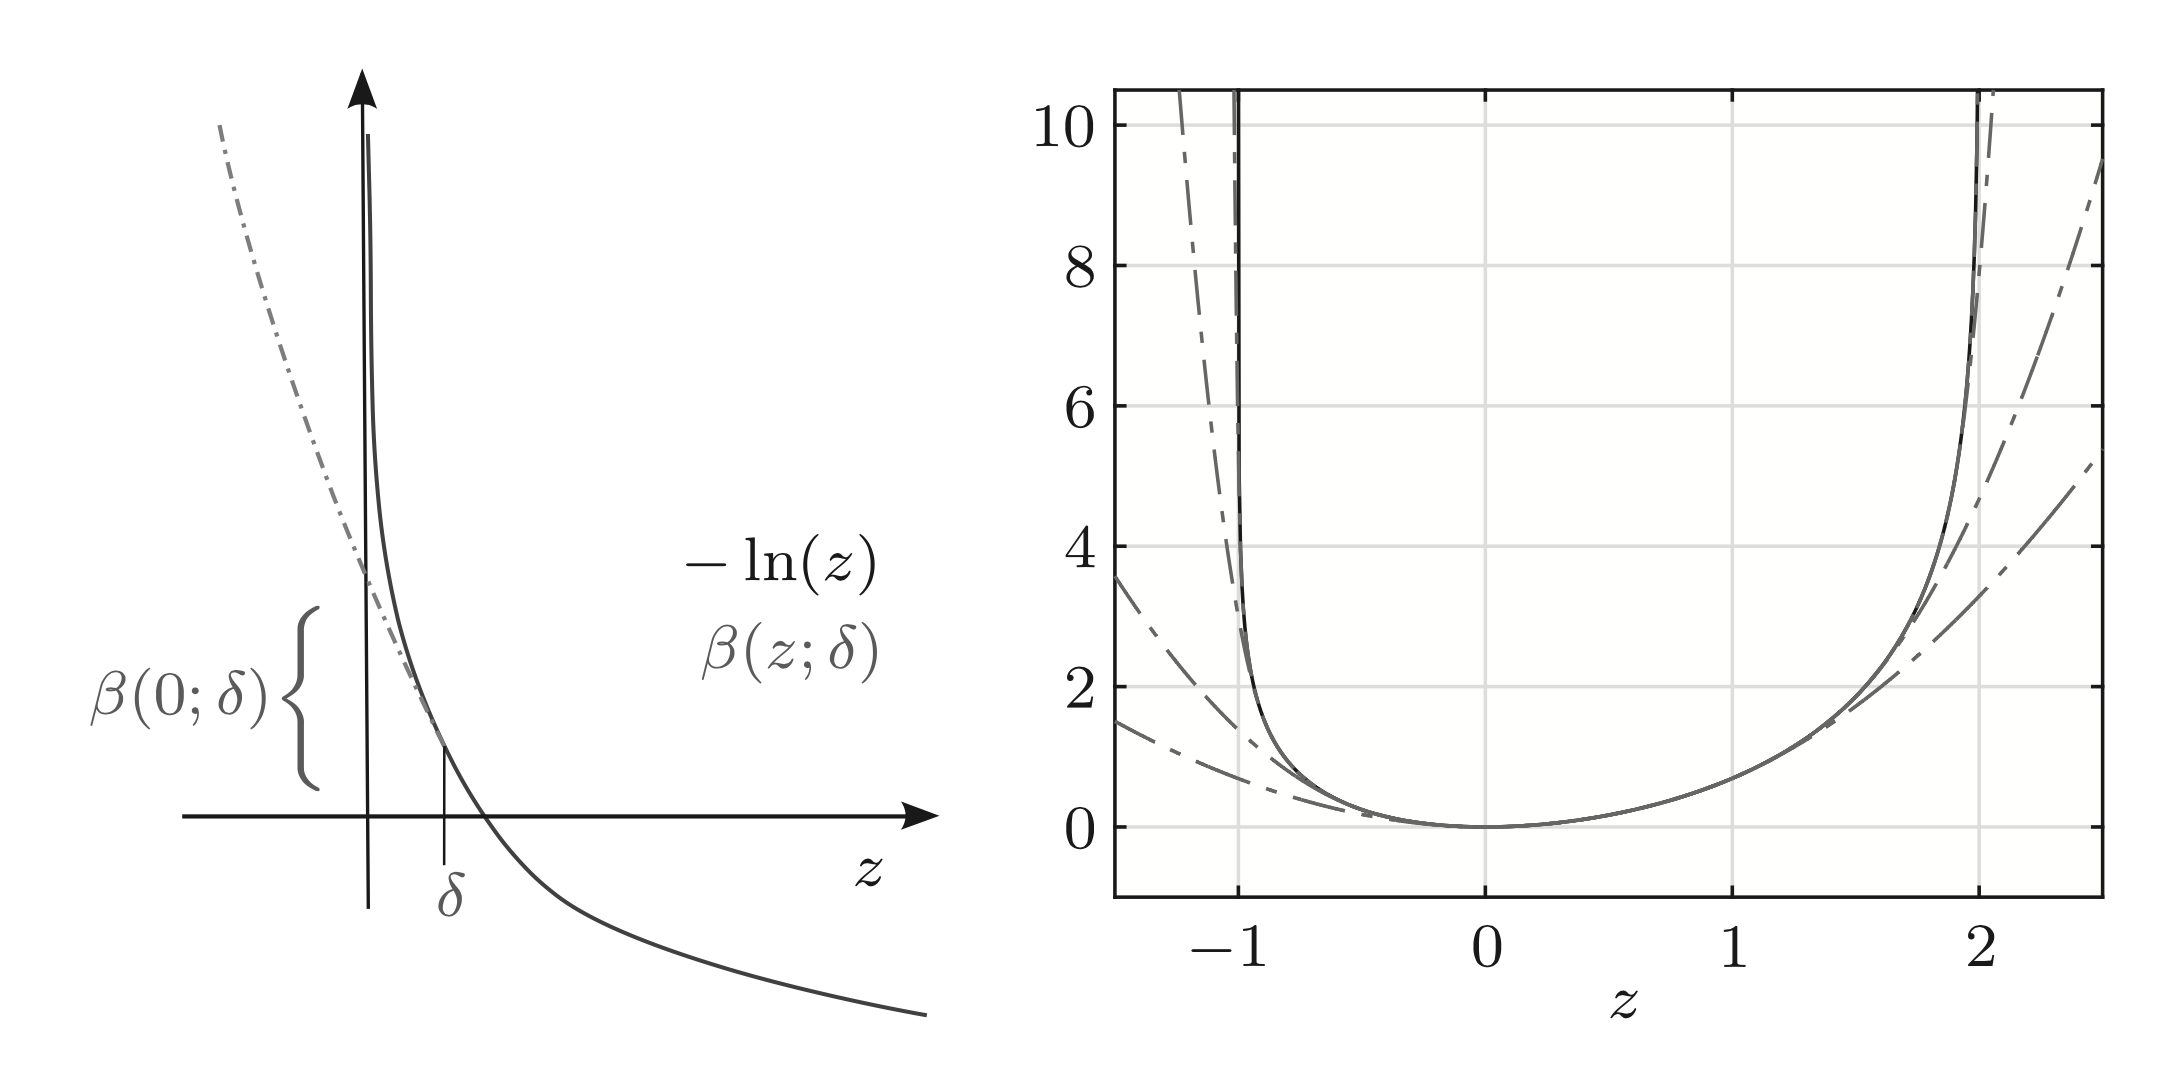
\includegraphics[width=0.8\textwidth]{images/rrlb-functions.png}
	\caption{\textit{(Left)}: Principle of relaxed log barrier function based on quadratic relaxation. (\textit{Right}): Regular weight recentered log barrier function (solid line) and RRLB function for $\delta\in\left\{ 0.01,0.1,0.5,1 \right\}$ for the constraint $z\in\R,~-1\leq z\leq 2$}
	\label{fig:RRLB-functions}
\end{figure}

\vspace{24pt}

\noindent With all these definitions we can finally define the \textit{RRLB MPC}:
\begin{align}
	\begin{split}\label{eq:RRLB-NMPC}
		\tilde{V}_N(x)=\underset{\bf{x},\bf{u}}{\min} &\quad \tilde{J}_N(\bf{x},\bf{u})\\
		\text{s.t.} &\quad x_0=x\text{ and }x_{k+1}=f(x_k,u_k),~k=0,\ldots,N-1\\
	\end{split}
\end{align}
where the new objective function $\tilde{J}_N(\bf{x},\bf{u})=\sum_{k=0}^{N-1}\tilde{l}(x_k,u_k)~+~\tilde{F}(x_N)$ is defined using the new stage costs $\tilde{l}(x,u)=l(x,u)+\epsilon B_x(x)+\epsilon B_u(u)$ and the new terminal cost $\tilde{F}(x)=x^TPx$ for another matrix $P$ that will be determined in such a way that the control law given by the MPC yields an asymptotically stable system.
The barrier parameter $\epsilon$ has in theory the following interpretation: when it goes to zero, the solution of problem~\ref{eq:RRLB-NMPC} converges to the one of~\ref{eq:NMPC}.
However, we will here consider it as fixed for simplicity.

\vspace{12pt}

\noindent When we consider the RRLB MPC~\ref{eq:RRLB-NMPC} in the case of linear dynamics $x^+=Ax+Bu$, we know the two following theorems.

\begin{theorem}[Theorem 5 in \cite{RRLB-linear-MPC}]
	\label{nominal-stability-linear-case}
	Suppose that the pair $(A,B)$ is stabilizable (the definition can be found in appendix~\ref{sec:controllability-stabilizability})
	and that the matrix $P$ is chosen as the unique positive definite solution to the following modified DARE:
	$$P=A^TPA-A^TPB(R+\epsilon M_u+B^TPB)^{-1}B^TPA+Q+\epsilon M_x$$
	where $M_x=\nabla^2 B_x(0)$ and $M_u=\nabla^2 B_u(0)$\, are the hessian of the RRLB functions at the origin.

	Then for any initial state $x(0)\in\R^{n_x}$, the control law given by the MPC yields an asymptotically stable system.
	% TODO: add definition of stabilizable
\end{theorem}

\begin{theorem}[Lemma 5 in \cite{RRLB-linear-MPC}]
	\label{constraint-satisfaction-guarantee-linear-case}
	In the same conditions as in the previous theorem, there is a neighborhood $\cal{X}_N(\delta)$ of the origin such that for any initial state $x(0)\in\cal{X}_N(\delta)$, all the constraint will be satisfied along the closed-loop trajectories.
	Furthermore, the set $\cal{X}_N(\delta)$ is given explicitly by:
	$$\cal{X}_N(\delta)=\left\{x\in\cal{X}~|~\tilde{V}_N(x(0))-x(0)^TP_{\rm{LQR}}x(0)\leq\min\{\beta_x(\delta),\beta_u(\delta)\}\right\}$$
	where $P_{\rm{LQR}}$ is the solution to the classical DARE~\ref{eq:DARE-LQR} and
	$$\beta_x(\delta)=\underset{i,x}{\min}\left\{ B_x(x)~|~\rm{row}_i(C_xx)=d_{x,i} \right\},\quad \beta_u(\delta)=\underset{i,u}{\min}\left\{ B_u(u)~|~\rm{row}_i(C_uu)=d_{u,i} \right\}$$
\end{theorem}

\noindent Additional results were proven in the linear case, such as the existence of a procedure to find $\delta$ such that the maximum constraint violation along the closed-loop trajectories is bounded by a pre-defined tolerance.
In the nonlinear case, however, we will not be able to prove such powerful results because of the lack of knowledge on the error terms that appear in the dynamics (see subsection~\ref{sec:constraints-satisfaction-guarantees}).

\section{Theoretical properties of RRLB Nonlinear MPC}\label{sec:RRLB-theoretical-properties}

In this section, we consider the RRLB MPC~\ref{eq:RRLB-NMPC} with nonlinear dynamics and show that the results of the previous section hold locally, in a neighborhood of the origin.

From this point on, for an initial state $x\in\R^{n_x}$ we will denote by \newline
$\tilde{\bf{x}}(x)=\left\{ \tilde{x}_0(x)=x,\tilde{x}_1(x),\ldots,\tilde{x}_N(x) \right\}$ and $\tilde{\bf{u}}(x)=\left\{ \tilde{u}_0(x),\tilde{u}_1(x),\ldots,\tilde{u}_{N-1}(x) \right\}$ the optimal sequences of states and controls found by the RRLB MPC.
When no confusion is possible we will drop the "$(x)$".

\subsection{Nominal asymptotic stability}\label{sec:RRLB-nominal-stability}

\begin{lemma}
	\label{thm:Lipschitzianity}
	Consider the RRLB MPC~\ref{eq:RRLB-NMPC} and re-write it in a simpler way as
	$$\tilde{V}_N(x)=\underset{\bf{u}}{\min} \quad J(x,\bf{u})$$
	where $J(x,\bf{u})=\tilde{l}(x,u_0)+\tilde{l}(f(x,u_0),u_1)+\cdots+\tilde{F}(f(f(...),u_{N-1}))$\,.
	If for a certain initial state $\bar{x}$ we suppose that $D_\bf{u}J(\bar{x},\tilde{\bf{u}})=0$ and $\nabla_{\bf{u}\bf{u}}^2J(\bar{x}, \tilde{\bf{u}})\succ 0$ (the matrix is positive definite) then in a neighborhood of $\bar{x}$ we have:
	\begin{itemize}[label=\textbullet]
		\item $\forall k=0,\ldots,N-1,\quad \|\tilde{u}_k(x)\|=O(\|x\|)$
		\item $\forall k=1,\ldots,N,\quad \|\tilde{x}_k(x)\|=f(f(\ldots,u_{k-2}),u_{k-1})=O(\|x\|)$
	\end{itemize}
\end{lemma}
\begin{proof}
	We can use the proof of the Theorem 4.2 in \cite{lectures-parametric-optimization} to argue that each $\tilde{x}_k$ and $\tilde{u}_k$ is continuously differentiable in a closed neighborhood of the origin.
	Therefore, by continuity their gradient is bounded on this neighborhood and they are Lipschitz.
\end{proof}

\noindent Now our main result:

\begin{theorem}\label{thm:nominal-stability}
	Let's consider the problem~\ref{eq:RRLB-NMPC} and assume the following:
	\begin{enumerate}
		\item If we denote the objective function as $J(x,\bf{u})$ as in Lemma~\ref{thm:Lipschitzianity}, we have $D_\bf{u}J(0,\bf{u}(0))=D_\bf{u}J(0,0)=0$ and $\nabla^2_{\bf{u}\bf{u}}J(0,\bf{u}(0))=\nabla^2_{\bf{u}\bf{u}}J(0,0)\succ 0$

		\item When linearizing the system dynamics around the equilibrium and letting $A=D_xf(0,0),$ $B=D_uf(0,0)$, we suppose that the pair $(A,B)$ is stabilizable (the definition can be found in appendix~\ref{sec:controllability-stabilizability}).
		This implies in particular that there exists a stabilizing cost $K$, i.e. a matrix such that $A_K:=A+BK$ only has eigenvalues in the unit disk.

		\item The matrix $P$ defining the terminal costs is the unique positive definite solution to the following Lyapunov equation:
		\begin{equation*}
			P=A_K^TPA_K+\mu Q_K
		\end{equation*}
		where $\mu>1$ and $Q_K=Q+\epsilon M_x+K^T(R+\epsilon M_u)K$\,.
	\end{enumerate}
	Then the dynamical system $x^+=f(x,\tilde{u}_0(x))$ is LAS, i.e. for all initial state in a neighborhood of the origin, the control law given by the RRLB MPC yields an asymptotically stable system.
\end{theorem}

\begin{remark}~
	The matrix $K$ can be constructed using the DARE for the following modified infinite horizon LQR problem:
	\begin{align}
		\begin{split}\label{eq:inf-LQR}
			\underset{\bf{x},\bf{u}}{\min} &\quad \sum_{k=0}^\infty x_k^T(Q+\epsilon M_x)x_k+u_k^T(R+\epsilon M_u)u_k\\
			\text{s.t.} &\quad x_{k+1}=Ax_k+Bu_k,~k=0,\ldots,N-1\\
		\end{split}
	\end{align}
	where $M_x=\nabla^2B_x(0)$ and $M_u=\nabla^2B_u(0)$, i.e.
	$$\begin{cases}
		K=-(R+B^T\Pi B)^{-1}B^T\Pi A&\\
		\Pi=A_K^T\Pi A_K+Q_K
	\end{cases}$$
	The only difference between this last equation and the Lyapunov equation in the statement of the theorem is the $\mu$ term.
	In theory it is very important, but in practice, we can actually take it very close to 1 and find $P$ and $K$ by solving
	$$\begin{cases}
		K=-(R+B^TP B)^{-1}B^TP A&\\
		P=A_K^TP A_K+Q_K
	\end{cases}$$
	More on that in~\ref{sec:RRLB-numerical-experiments}.
\end{remark}

\begin{proof}~
	To prove the result we will show that $\tilde{V}_N$ is a Lyapunov function in a neighborhood of the origin.
	First, by writing the Taylor expansion of the stage costs $\tilde{l}$ we can see that
	\begin{align*}
		\tilde{l}(x,u)&=x^T[\nabla_{xx}^2\tilde{l}(0,0)] x+u^T[\nabla_{uu}^2\tilde{l}(0,0)]u+O(\|x\|^3+\|u\|^3)\\
		&=x^T[Q+\epsilon M_x]x+u^T[R+\epsilon M_u]u+O(\|x\|^3+\|u\|^3)
	\end{align*}
	so $\tilde{l}(x,Kx)=x^TQ_Kx+O(\|x\|^3)$\,.
	By the second assumption, we also have $\forall x\in\R^{n_x}$:
	$$\tilde{F}(A_Kx)+\mu x^T Q_K x-\tilde{F}(x)=0$$
	We can use the same reasoning as in the paragraph 2.5.5 of \cite{MPC-book} to show that $\tilde{F}$ is a local Lyapunov function, i.e. there exists a neighborhood of the origin such that $\forall x$ in it:
	$$\tilde{F}(f(x,Kx))+x^T Q_K x-\tilde{F}(x)\leq 0\Longrightarrow\tilde{F}(f(x,Kx))-\tilde{F}(x)+\tilde{l}(x,Kx)=O(\|x\|^3)$$

	\noindent What's more, by previous lemma, the predicted states are all Lipschitz with respect to the initial state, so we can choose an even smaller neighborhood such that $\tilde{x}_N(x)$ is also in it.

	\noindent Now using the optimal sequence of states and controls of the RRLB MPC starting at $x$, we can construct new feasible sequences for the problem starting at $\tilde{x}_1(x)$ as \newline
	$\bf{x}'=(\tilde{x}_1,\ldots,\tilde{x}_N,f(\tilde{x}_N,K\tilde{x}_N))$ and $\bf{u}'=(\tilde{u}_1,\ldots,\tilde{u}_{N-1},K\tilde{x}_N)$\,.
	Then we have:
	$$\tilde{V}_N(\tilde{x}_1)\leq\tilde{J}_N(\bf{x}',\bf{u}')=\underbrace{\tilde{J}_N(\tilde{\bf{x}},\tilde{\bf{u}})}_{=\tilde{V}_N(x)}~\underbrace{\underbrace{-\tilde{l}(x,\tilde{u}_0)}_{=O(\|x\|^2)}+\underbrace{\tilde{F}(f(\tilde{x}_N,K\tilde{x}_N))-\tilde{F}(\tilde{x}_N)+\tilde{l}(\tilde{x}_N,K\tilde{x}_N) }_{=O(\|\tilde{x}_N\|^3)=O(\|x\|^3)} }_{\leq-c\|x\|^2\text{ in a smaller nbh }}\checkmark$$
	We have therefore shown the descent property of our candidate Lyapunov function $\tilde{V}_N$\,.
	Finally, it is easy to show that $\tilde{V}_N$ is lower and upper bounded by coercive quadratic functions (since $Q,R$ are positive definite and $B_x,B_u$ are positive definite and upper bounded by quadratics), so that $\tilde{V}_N$ is indeed a Lyapunov function in a small neighborhood around the origin.
\end{proof}

\subsection{Constraints satisfaction guarantees}\label{sec:constraints-satisfaction-guarantees}
This section follows closely the section IV.D of \cite{RRLB-linear-MPC} but gives more loose results that cannot take us as far.
In particular, will show that we can ensure the existence of a neighborhood around the origin such that if we start in it, the states and controls along the closed-loop trajectories will never violate the constraints.
However, this neighborhood cannot be easily computed because of the generality of the considered dynamics, and will therefore not be verified experimentally in section~\ref{sec:RRLB-numerical-experiments}.
In the whole section, we assume Theorem~\ref{thm:nominal-stability} to hold.

\begin{lemma}
	\label{thm:RRLB-bounds-guarantees}
	Consider the RRLB MPC~\ref{eq:RRLB-NMPC} and an initial state $x(0)$ in the neighborhood given by Theorem~\ref{thm:nominal-stability}.
	Let's denote by $\left\{x(0),x(1),\ldots\right\}$ and $\left\{u(0), u(1),\ldots\right\}$ the closed-loop state and control trajectories (given by $u(k)=\tilde{u}_0(x(k)),~x(k+1)=f(x(k),u(k))$).
	Then $\forall k\geq 0$:
	\begin{align*}
		B_x(x(k))&\leq\frac{1}{\epsilon}\left(\tilde{V}_N(x(0))-x(0)^TP_{\rm{LQR}}x(0)-\sum_{k=0}^\infty\eta(x(k))\right)\\
		B_u(u(k))&\leq\frac{1}{\epsilon}\left(\tilde{V}_N(x(0))-x(0)^TP_{\rm{LQR}}x(0)-\sum_{k=0}^\infty\eta(x(k))\right)
	\end{align*}
	where $P_{\rm{LQR}}$ is the solution to the DARE associated to~\ref{eq:inf-LQR} and $\eta(x)=\tilde{l}(\tilde{x}_N(x),K\tilde{x}_N(x))+\tilde{F}(\tilde{x}_N(x))-\tilde{F}(f(\tilde{x}_N(x), K\tilde{x}_N(x)))$.
\end{lemma}

\begin{proof}
	In the proof of theorem~\ref{thm:nominal-stability} we showed that $\forall k\geq 0$:
	\begin{multline*}
		\tilde{V}_N(x(k+1))-\tilde{V}_N(x(k))\leq-\tilde{l}(x(k),u(k))+\tilde{l}(\tilde{x}_N(x(k)), K\tilde{x}_N(x(k)))\\
		-\tilde{F}(\tilde{x}_N(x(k)))+\tilde{F}(f(\tilde{x}_N(x(k)),\tilde{x}_N(x(k))))
	\end{multline*}
	so by summing everything we get a telescopic sum that we can compute using the fact that the system is asymptotically stable so $\lim_{k\to\infty}\tilde{V}_N(x(k))=0$, we get:
	\begin{align*}
		\tilde{V}_N(x(0))&\geq\sum_{k=0}^\infty\tilde{l}(x(k),u(k))-\tilde{l}(\tilde{x}_N(x(k)), K\tilde{x}_N(x(k)))+\tilde{F}(\tilde{x}_N(x(k)))-\tilde{F}(f(\tilde{x}_N(x(k)),\tilde{x}_N(x(k))))\\
		&=\sum_{k=0}^\infty l(x(k), u(k))+\epsilon B_x(x(k))+\epsilon B_u(u(k))+\eta(x(k))\\
		&\geq x(0)^TP_{\rm{LQR}}x(0)+\sum_{k=0}^\infty\eta(x(k))+\epsilon\sum_{k=0}^\infty B_x(x(k))+\epsilon\sum_{k=0}^\infty B_u(u(k))\\
	\end{align*}
	Even if we don't know a closed form for $\eta(x(k))$, we know that $\sum_{k=0}^\infty\eta(x(k))$ must be finite because it is bounded by $\tilde{V}_N(x(0))$\,.
	Now since the RRLB functions are all positive definite, we can easily conclude.
\end{proof}

We define for ease of notation the following quantities
\begin{align*}
	\alpha(x(0))&=\tilde{V}_N(x(0))-x(0)^TP_{\rm{LQR}}x(0)-\sum_{k=0}^\infty\eta(x(k))\\
	\beta_x&=\underset{i,x}{\min}\{B_x(x)~|~\rm{row}_i(C_x)x=d_{x,i}\}\\
	\beta_u&=\underset{i,u}{\min}\{B_u(u)~|~\rm{row}_i(C_u)u=d_{u,i}\}
\end{align*}

Even if not written explicitly, the bounds $\beta_x,\beta_u$ depend on the relaxation parameter $\delta$\,.

\begin{lemma}
	\label{thm:constraint-set-def-with-RRLB}
	For all relaxation parameter $\delta$:
	$$\left\{x\in\R^{n_x}~|~B_x(x)\leq\beta_x\right\}\subseteq\cal{X},\quad\left\{u\in\R^{n_u}~|~B_u(u)\leq\beta_u\right\}\subseteq\cal{U}$$
\end{lemma}

\begin{proof}
	See Lemma 1 in \cite{RRLB-linear-MPC}.
\end{proof}

\begin{theorem}
	In the same setting as lemma~\ref{thm:RRLB-bounds-guarantees}, for any initial state $x(0)$ in the set
	$$\cal{X}_N(\delta):=\left\{x\in\R^{n_x}~|~\alpha(x(0))\leq\epsilon\min\left\{\beta_x,\beta_u\right\}\right\}$$
	there is no state or control constraint violation along the closed loop trajectories.
\end{theorem}

\begin{proof}
	For any $x(0)\in\cal{X}_N(\delta)$ it holds due to~\ref{thm:RRLB-bounds-guarantees} that for all $k\geq 0,~\epsilon B_x(x(k))\leq\alpha(x(0))\leq\epsilon\beta_x$ so $B_x(x(k))\leq \beta_x$ and $x(k)\in\cal{X}$.
	The same reasoning applies on the controls.
\end{proof}

% \newpage

\section{Numerical aspects of RRLB}\label{sec:RRLB-numerical-aspects}

In this section we take a more concrete look at the numerical methods employed to solve MPC problems in practice.
One of the more important challenges of such implementations resides in the large number of variables and more generally the complexity of the NLP to be solved, that may not permit finding an accurate solution when the sampling time is very short.
This issue is deeply aggravated on embedded platforms where the computational power is often limited.
This is why, historically, the first successful implementations of MPC in industrial applications were found in chemical engineering, where the sampling time (duration between two state measurement, and therefore time available to compute a new control) are usually long enough to find an accurate solutions.
For instance, in the chemical system studied in subsection~\ref{sec:RRLB-numerical-experiments}, the sampling time is of $200.0s$, while in robotics or autonomous driving the sampling time is rather in the order of the $10.0ms$.

A great deal of effort has been put in the past decade to design algorithms that make best use of scarce computational power to deliver usable results on embedded systems that necessitate very fast response times.
One that rapidly gained interest is a variant of \textit{Sequential Quadratic Programming} (or SQP) called \textit{Real Time Iteration} (or RTI).
Invented by Moritz Diehl and published in \cite{rti-diehl}, it can roughly be defined as SQP with a fixed number of iterations, usually only one, that makes use of the solutions found at the previous MPC prediction to warm-start the solver and to ensure both computational efficiency and accuracy.

In subsection~\ref{sec:RTI-scheme} we formally introduce the RTI scheme for general MPC and the specialize it for RRLB MPC, then briefly discuss it stability properties in subsection~\ref{sec:RRLB-real-time-stability} and finally present numerical results verifying the theoretical properties of RRLB MPC and compare its performance with regular MPC in subsection~\ref{sec:RRLB-numerical-experiments}.

\subsection{The RTI scheme}\label{sec:RTI-scheme}

We assume in this section familiarity with the SQP framework for general NLPs, as described for example in \cite{nocedal-wright}, and describe it in the context of MPC.
We don't explicitly deal with the assumptions necessary for SQP to converge.
% TODO: do we really ignore them ?

\subsubsection{SQP for regular MPC}

Just as in sections~\ref{sec:RRLB-MPC} and~\ref{sec:RRLB-theoretical-properties}, we are going to consider the target state and controls to be the origin, which will simplify our notations inspired from \cite{mpc-rti}.
With the following general MPC:

\begin{align*}
	\mathrm{MPC}(x)=\underset{\bf{x},\bf{u}}{\min} &\quad \sum_{k=0}^{N-1}l(x_k,u_k)~+~F(x_N)\\
	\text{s.t.} &\quad x_0=x\text{ and }x_{k+1}=f(x_k,u_k),~k=0,\ldots,N-1\\
	&\quad h_x(x_k)\leq 0,~k=0,\ldots,N\\
	&\quad h_u(u_k)\leq 0,~k=0,\ldots,N-1
\end{align*}

\noindent we can define the following QP subproblem:

\begin{align*}
	\mathrm{QP}(x, \mathbf{x}_i, \mathbf{u}_i)=\underset{\Delta\mathbf{x}_i,\Delta\mathbf{u}_i}{\mathrm{argmin}} & \quad \sum_{k=0}^{N-1}\begin{pmatrix}\Delta x_{i,k}\\\Delta u_{i,k}\end{pmatrix}^TH_{i,k}\begin{pmatrix}\Delta x_{i,k}\\\Delta u_{i,k}\end{pmatrix}+J_{i,k}^T\begin{pmatrix}\Delta x_{i,k}\\\Delta u_{i,k}\end{pmatrix}\\
	&\quad +\Delta x_{i,N}^TH_{i,N}\Delta x_{i,N}+J_{i,N}^T\begin{pmatrix}\Delta x_{i,N}\\\Delta u_{i,N}\end{pmatrix}\\
	\text{s.t.} &\quad \Delta x_0=x-x_{i,0}\\
	&\quad \Delta x_{i,k+1}=A_{i,k}\Delta x_{i,k}+B_{i,k}\Delta u_{i,k}+r_{i,k},~k=0,\ldots,N-1\\
	&\quad C_{i,k}\Delta x_{i,k}+h_{x,i,k}\leq 0,~k=0,\ldots,N\\
	&\quad D_{i,k}\Delta x_{i,k}+h_{u,i,k}\leq 0,~k=0,\ldots,N-1
\end{align*}

\noindent with the sensitivities:

\begin{align*}
		&A_{i,k}=D_xf(x_{i,k}, u_{i,k}),~B_{i,k}=D_uf(x_{i,k}, u_{i,k}),~C_{i,k}=D_xh(x_{i,k}, u_{i,k}),~D_{i,k}=D_uh(x_{i,k}, u_{i,k})\\
		&J_{i,k}=\nabla l(\Delta x_{i,k},\Delta u_{i,k}),~J_{i,N}=\nabla F(\Delta x_N)\\
		&r_{i,k}=f(x_{i,k}, u_{i,k})-x_{i,k+1},\quad h_{x,i,k}=h_x(x_{i,k}),\quad h_{u,i,k}(u_{i,k})
\end{align*}

\noindent and $H_{i,k}\approx \nabla^2_{(x_k,u_k),(x_k,u_k)}\calL(\mathbf{x}_i,\mathbf{u}_i),~H_{i,N}\approx\nabla^2_{x_N,x_N,u_N}\calL(\mathbf{x}_i,\mathbf{u}_i)$, where $\calL$ is the Lagrangian of the MPC problem.

When using quadratic stage and terminal costs and when we choose to use Gauss-Newton approximation for the Hessian, we get:
\begin{equation*}
	H_{i,k}=\begin{pmatrix}Q&0\\0&R\end{pmatrix},\quad H_{i,N}=P,\quad J_{i,k}=\begin{pmatrix}Q&0\\0&R\end{pmatrix}\begin{pmatrix}\Delta x_{i,N}\\\Delta u_{i,N}\end{pmatrix},\quad J_{i,N}=P\begin{pmatrix}\Delta x_{i,N}\\\Delta u_{i,N}\end{pmatrix}
\end{equation*}

\noindent What's more, when the constraints are polytopic, the sensitivities read:

\begin{equation*}
	C_{i,k}=C_x,~D_{i,k}=C_u,~h_{x,i,k}=C_xx_{i,k}-d_x,~h_{u,i,k}=C_uu_{i,k}-d_u
\end{equation*}

These two particular cases make up the MPC we have been studying in this whole paper, that we will call in this section the \textit{regular MPC}.


\noindent With all these definitions, the complete SQP method reads:

\begin{algorithm}[H]
	\caption{SQP method for regular MPC}
	\label{algo:SQP-reg}
	\begin{algorithmic}[1]
	\Procedure{SQP}{x, $\mathbf{x}^{init}$, $\mathbf{u}^{init}$}
	\State{$\mathbf{x}_0\gets\mathbf{x}^{init}$} \Comment{initial guess for the states specified by the user}
	\State{$\mathbf{u}_0\gets\mathbf{u}^{init}$} \Comment{initial guess for the controls specified by the user}
	\State{$k\gets 0$}
	\While{a stopping cirterion is not met}\\
		\qquad \quad Compute $r_{i,k}, h_{x,i,k}, h_{u,i,k}$ and the sensitivities $A_{i,k}, B_{i,k}, C_{i,k}, D_{i,k}$ as above
		\State{$(\Delta\mathbf{x}_i, \Delta\mathbf{u}_i)\gets \mathrm{QP}(x, \mathbf{x}_i, \mathbf{u}_i)$} \Comment{Find descent direction as above}
		\State{$\mathbf{x}_{i+1}\gets\mathbf{x}_i+\Delta\mathbf{x}_i$}
		\State{$k\gets k+1$}
	\EndWhile
	\EndProcedure
	\end{algorithmic}
\end{algorithm}

\subsubsection{SQP for RRLB MPC}

Using the same notations as above, the only things that change are the fact that the inequality constraints are ignore and that the sensitivities are computed in the following way:

\begin{align*}
	&H_{i,k}=2\begin{pmatrix}Q&0\\0&R\end{pmatrix}+\epsilon\begin{pmatrix}\nabla^2B_x(x_{i,k})&0\\0&\nabla^2B_u(u_{i,k})\end{pmatrix},\quad H_{i,N}=P+\epsilon\nabla B_x(x_{i,N})\\
	&J_{i,k}=2\begin{pmatrix}Q&0\\0&R\end{pmatrix}\begin{pmatrix} x_{i,k}\\ u_{i,k}\end{pmatrix}+\epsilon\begin{pmatrix}\nabla B_x(x_{i,k})\\\nabla B_u(u_{i,k})\end{pmatrix},\quad J_{i,N}=2P x_{i,N}+\epsilon\nabla B_x(x_{i,N})
\end{align*}

\subsubsection{Remarks on SQP}

In \cite{mpc-rti} the presented SQP procedure includes a line-search step that computes a step size $\alpha\in(0,1]$ such that enough progress is made at each iteration.
In the case of general SQP, this is particularly important to ensure convergence.
However, if the initial guesses $\mathbf{x}^{init},~\mathbf{u}^{init}$ are well chosen, we can take full steps at each iteration and therefore attain faster convergence.

The most natural way to construct this initial guess would be to \textit{shift} the solution found at the previous control update (or equivalently, at the previous call to the solver of algorithm~\ref{algo:SQP-reg}).
More precisely, if at time $k$ we found $\mathbf{x}=(x_0,\ldots,x_N),\mathbf{u}=(u_0,\ldots,u_{N-1})$ then our initial guess at time $k+1$ will be $\mathbf{x}^{init}=(x_1,\ldots,x_N,f(x_N,u_{new})),\mathbf{u}^{init}=(u_1,\ldots,u_{N-1},u_{new})$ where $u_new$ might be chosen using different strategies:
\begin{itemize}[label=\textbullet]
	\item whenever possible, setting $u_{new}=\kappa(x_N)$ where $\kappa:\cal{X}\to\cal{U}$ is a \textit{locally stabilizing control law} that would make converge to the origin all the states in a neighborhood, without taking into account the constraints.
	An example of such locally stabilizing control law can be the control law of the infinite horizon LQR mentioned in subsection~\ref{sec:what-is-MPC}.

	\item using the reference control $u^*$ (which again we consider as $0$ for simplicity).

 	\item using the same control as in the previous stage: $u_{new}=u_{N-1}$\,.
\end{itemize}

This shifting heuristic is based on the fact that the dynamics $f$ should either exactly equal or at least close to the actual dynamics of the system so that this initial guess is very close to the actual solution.
When it is the case, and if the solution found at time $k$ is feasible, then so will be the initial guess for time $k+1$, and the very first iteration of algorithm~\ref{algo:SQP-reg} provides a very accurate estimate of the solution at time $k+1$.
Numerical illustrations of these statements can be found in \cite{mpc-rti}.
This method supposes that the very first prediction of a closed-loop experiment has to be computed exactly, but this can be done offline (i.e. before starting the simulation) with an arbitrary accuracy.

\subsubsection{The RTI scheme}

RTI relies on previous remarks to find an accurate solution to the MPC problem and combines them with another important idea trying to solve the \textit{real-time dilemma} which can be summarized in the following way:

\begin{quote}
	Upon obtaining a new state estimate $x$, a new SQP procedure can be started to find the solution of the MPC.
	During the execution, the systems continues to evolve and by the time it finishes, the current state of the system won't be the one fed to the algorithm, making the prediction obsolete.
\end{quote}

To overcome this issue, RTI separates the SQP procedure into:
\begin{itemize}[label=\textbullet]
	\item a \color{red}{\textit{preparation phase}}\color{black}~comprising the computation of the sensitivities and the condensation (i.e. the creation of the sparse matrices defining the QP problem by concatenating the terms of each stage) and

	\item a \color{blue}\textit{feedback phase}\color{black}~that solves the QP using the last available state estimate as initial state.
\end{itemize}

This makes sense, since the preparation phase only actually needs information from the previous call to the solver, and can therefore be started right after it, before the next state estimate is even available.

Instead of presenting RTI with pseudocode as in algorithm~\ref{algo:SQP-reg}, we will rather draw up a timeline resuming how the different steps of the algorithm are used in real situation:

\vspace{12pt}

\begin{figure}[H]
	\startchronology[startyear=-3,stopyear=5,startdate=false,dates=false,color=black,width=\textwidth, arrow=true]
	\chronoperiode[color=cyan, dates=false]{-3}{0}{\textcolor{cyan}{off-line initialization}}
	\chronoevent[year=false]{0}{\color{green}{m}}
	\chronoperiode[color=red,datesstyle={t},stopdate=false]{0}{1}{\textcolor{red}{P}}
	\chronoevent[year=false]{1}{\color{green}{m}}
	\chronoperiode[color=blue,datesstyle={t},stopdate=false]{1}{2}{\textcolor{blue}{F}}
	\chronoevent[year=false]{2}{}
	\chronoperiode[color=red,datesstyle={t},stopdate=false]{2}{3}{\textcolor{red}{P}}
	\chronoevent[year=false]{3}{\color{green}{m}}
	\chronoperiode[color=blue,datesstyle={t},stopdate=false]{3}{4}{\textcolor{blue}{F}}
	\chronoevent[year=false]{4}{}
	\chronoperiode[color=red,datesstyle={t}]{4}{5}{\textcolor{red}{P}}
	\chronoevent[year=false]{5}{\color{green}{m}}
	\stopchronology
	\caption{RTI timeline}
	\label{fig:RTI-timeline}
\end{figure}

\noindent Several important points should be highlighted:

\begin{itemize}[label=\textbullet]
	\item Before the start of the experiment, we solve the problem with an arbitrary precision \textbf{offline}, when there is no limit on the running time of the solver.
	This supposes that we know in advance the initial state of the system, but this is a common and realistic assumption.
	In this phase, we could use the general SQP with as many steps as necessary for full convergence (remember that we can't properly use RTI yet since we don't have a good initial guess), or any other algorithm to solver constrained NLPs.

	\item The "\color{green}m\color{black}" labels indicate the state measurements of the system.
	In practice, we suppose they are done at a constant rate given by the sampling time $dt$, and we can thus say that $\rm{t}1-\rm{t}0=dt$ and $\rm{t}(2k+3)-\rm{t}(2k+1)=dt,~\forall k\geq 0$\,.

	\item The phases denoted by "\color{red}P\color{black}" and "\color{blue}F\color{black}" are the preparation and feedback phases of the RTI scheme as described above.

	\item During the experiment, the state evolves continuously, but the control parameters are kept constant on all intervals of the form $[\rm{t}(2k),\rm{t}(2k+2))$ because we update the control only when a new one is computed.
\end{itemize}

More practical details on RTI will be given in subsection~\ref{sec:RRLB-numerical-experiments} where we apply this scheme to the simulation of a real system.
In particular, we will give explicit details on the form of the matrices to condense.

\subsection{Asymptotic stability of RTI scheme}\label{sec:RRLB-real-time-stability}

Section~\ref{sec:RRLB-theoretical-properties} proved several important theoretical properties of RRLB MPC, and the next subsection presents some experimental verifications of these theorems.
However, it should be noted that all the solution to problem~\ref{eq:RRLB-NMPC} found in these experiments are by essence inexact, and we can therefore not easily claim that the asymptotic stability and the constraint satisfaction still hold in practice. That's why we make the distinction between \textit{nominal stability} and \textit{real-time stability}.

The determination of assumptions and results guaranteeing these properties in the real-time framework have been studied for example by Moritz Diehl or Andrea Zanelli, although in slightly different contexts than ours.
The managed to derive powerful theorems but their assumptions are hard or even impossible to verify in practice and they are not really verified in practice.
Instead, the desired properties are verified experimentally by means of a simple simulation of the system at hand.
This is the scope of next subsection, in which we will not worry about this distinction between nominal and real-time stability.


\subsection{Numerical experiments}\label{sec:RRLB-numerical-experiments}

In this section, we verify the stability properties of the RRLB MPC using a concrete system that is often used to benchmark different MPC schemes or solvers: the Continuously Stirred Tank Reactor (CSTR).
We will not however determine explicitly the neighborhood given by theorem~\ref{thm:nominal-stability} because of the lack of theoretical description.
For the same reason, we will not compute the neighborhood given by theorem~\ref{thm:RRLB-bounds-guarantees}, and just see if the constraints are satisfied or not along the closed-loop trajectories.
When they are, this will allow us to explicitly compare RRLB to regular MPC.

\subsubsection{Experimental setup}

The CSTR system describes an exothermic chemical reaction with 4 states ($c_A$ the concentration of cyclopentadiene (reactant), $c_B$ the concentration of cyclopentenol (product), $\vartheta$ the temperature in the reactor and $\vartheta_K$ the temperature in the cooling jacket of the tank reactor) and 2 controls ($u_1$ the scaled feed inflow rate of cyclopentadiene and $u_2$ the heat removal rate of the external heat exchanger designed to cool down the reactor).
The system of ODEs describing the model as well as the costs and constraints can be found in the appendix~\ref{sec:cstr-model}, and more details about this system can be found in \cite{diehl-dissertation}.

By a simple steady state analysis procedure \footnote{This procedure was applied to the discrete-time dynamics obtained via discretization with RK4.}, we determined 3 viable reference points for states and controls that can be found (at $10^{-3}$ precision and in SI units) in table~\ref{tab:CSTR-ref-points}.

\begin{table}%[H]
	\centering
	\begin{tabular}{|c|c|c|c|c|c|c|}
		\hline
		Ref point & $c_A^*$ & $c_B^*$ & $\theta^*$ & $\theta_K^*$ & $u_1^*$ & $u_2^*$ \\
		\hline
		1 & 2.140 & 1.090 & 114.191 & 112.907 & 14.19 & -1113.50 \\
		\hline
		2 & 2.715 & 1.023 & 105.506 & 100.892 & 13.666 & -3999.589 \\
		\hline
		3 & 2.975 &  0.954 & 101.150 & 95.194 & 12.980 & -5162.957 \\
		\hline
	\end{tabular}
	\caption{Reference points for the CSTR system}
	\label{tab:CSTR-ref-points}
\end{table}

\noindent Some general remarks on the implementation:
\begin{itemize}[label=\textbullet]
	\item None of the reference points in table~\ref{tab:CSTR-ref-points} are 0, therefore we had to translate everything as briefly described at the beginning of section~\ref{sec:what-is-MPC}.

	\item The discrete-time dynamics have been obtained from the model's ODE by using a 6-step RK4 scheme.

	\item We chose a sampling time of $20.0s$, and variable horizon lengths between 25 and 250 time steps.
	In all our experiments we set the maximum number of control feedbacks to 350 and ran the simulation in closed loop (i.e. applying to the system the control computed by the MPC) until the state converged to the reference state within a $10^{-3}$ relative tolerance in norm (i.e. $\|x-x^*\|_\infty/\|x^*\|_\infty<10^{-3}$).

	\item For RRLB MPC, we determined the terminal cost by solving the modified DARE with $\mu=1$ as mentioned in~\ref{sec:RRLB-nominal-stability}.
	We will see in the results that this does not impact convergence when the horizon size is big enough.

	\item For RRLB MPC, the relaxation parameter $\delta$ was chosen as $\frac{1}{2}\min\left\{ d_{x,1},\ldots, d_{x,q_x},d_{u,1},\ldots,d_{u,q_u} \right\}$ and the barrier parameter $\epsilon$ was chosen as $1.0e-3$ after a bit of tuning in order to ensure that the MPC would converge.

	\item The initial prediction (as described in~\ref{sec:RTI-scheme}) is computed using the interior point method solver IPOPT (see \cite{ipopt}) through the algorithmic differentiation package CasADi (see \cite{casadi}).

	\item RTI was implemented from scratch using OSQP (see \cite{osqp}) to solve the quadratic subproblems.
	This library solves general quadratic problems of the form:
	\begin{align*}
		\underset{z\in\R^n}{\min}&\quad\frac{1}{2}z^TPz+q^Tz\\
		\text{s.t.}&\quad l\leq Az\leq u
	\end{align*}
	We therefore have to translate the QPs found in section~\ref{sec:RTI-scheme} for regular MPC and RRLB MPC into this form, which corresponds to the condensation part of the preparation phase.
	The exact form of the matrices and vectors involved in this formulation can be found in~\ref{sec:osqp-condensation}.

	\item The whole implementation for this project was done in Python and can be found in the folder \verb|cstr| attached to the project report.
	To test the code, we recommend creating a virtual environment using the \verb|requirements.txt| file provided.
	The code is heavily documented and general indications on the structure of the code are given in the \verb|README.md| file.
\end{itemize}

\subsubsection{Experimental procedure}

We generated a list of 5 random initial states (that can be found in the columns of the file \verb|exp_all_initial_states.csv| in the directory \verb|results|) using a uniform distribution between the following bounds:
$$0.0\leq c_A,c_B\leq 5.0,~98.0\leq\vartheta\leq 110.0,~92.0\leq \vartheta_K\leq 110.0$$
and with the 3 reference points in table~\ref{tab:CSTR-ref-points}, this generated 15 different situations in which we ran the following experiment:

We first ran an open loop simulation of the infinite horizon MPC (approximated by a regular MPC with horizon length of 5000) to determine an 'optimal' behavior\footnote{As described in section~\ref{sec:what-is-MPC}}, and then ran closed-loop simulations with RRLB MPC and regular MPC and variable horizon lengths for both of them (in the list $\left\{ 25, 50, 100, 250 \right\}$).
For all of them we measured:
\begin{itemize}[label=\textbullet]
	\item the \textit{performance measure}, i.e. the sum of the stage costs over all the time steps up until convergence, or the maximum number of time feedbacks, is reached.

	For the the closed loop simulations, RTI was used and the sum was only done over the time instants where a \textit{measurement is made} (see~\ref{fig:RTI-timeline}).

	\item the number of iterations taken to reach the convergence.

	\item whether the constraints were violated or not.
\end{itemize}

\noindent Additionally, for the closed-loop simulations where RTI was used, we also measured the times (average and standard error) in milliseconds of the sensitivity computation, the condensation, and the QP solve.
All these measures can be found in the file \verb|exp_all_results.csv| in the folder \verb|results|.

\subsubsection{Results and discussion}\label{sec:results-discussion}

\noindent From all the measures described above, we can make several observations:

\begin{itemize}[label=\textbullet]
	\item In every situation, when the horizon size is 25, the RRLB MPC does not manage to converge to the desired reference point and instead converges to another steady state.
	For instance, for initial state n°1 and reference point n°1, it converges to (values are given at $10^{-4}$ precision):
	$$x^*=(2.0005, 1.086, 117.3737, 117.5026),\quad u^*=(15.2094, 111.7617)$$
	Nonetheless, when decreasing the barrier parameter $\epsilon$, we can produce convergence at the expense of more constraint violation due to the fact that the constraints are somehow less enforced.
	The corresponding closed loop trajectories can be found in figure~\ref{fig:closedloop_traj_rrlb_1_1_25}.

	\begin{figure}[!hp]
		\centering
		\begin{subfigure}{15cm}
			\centering
			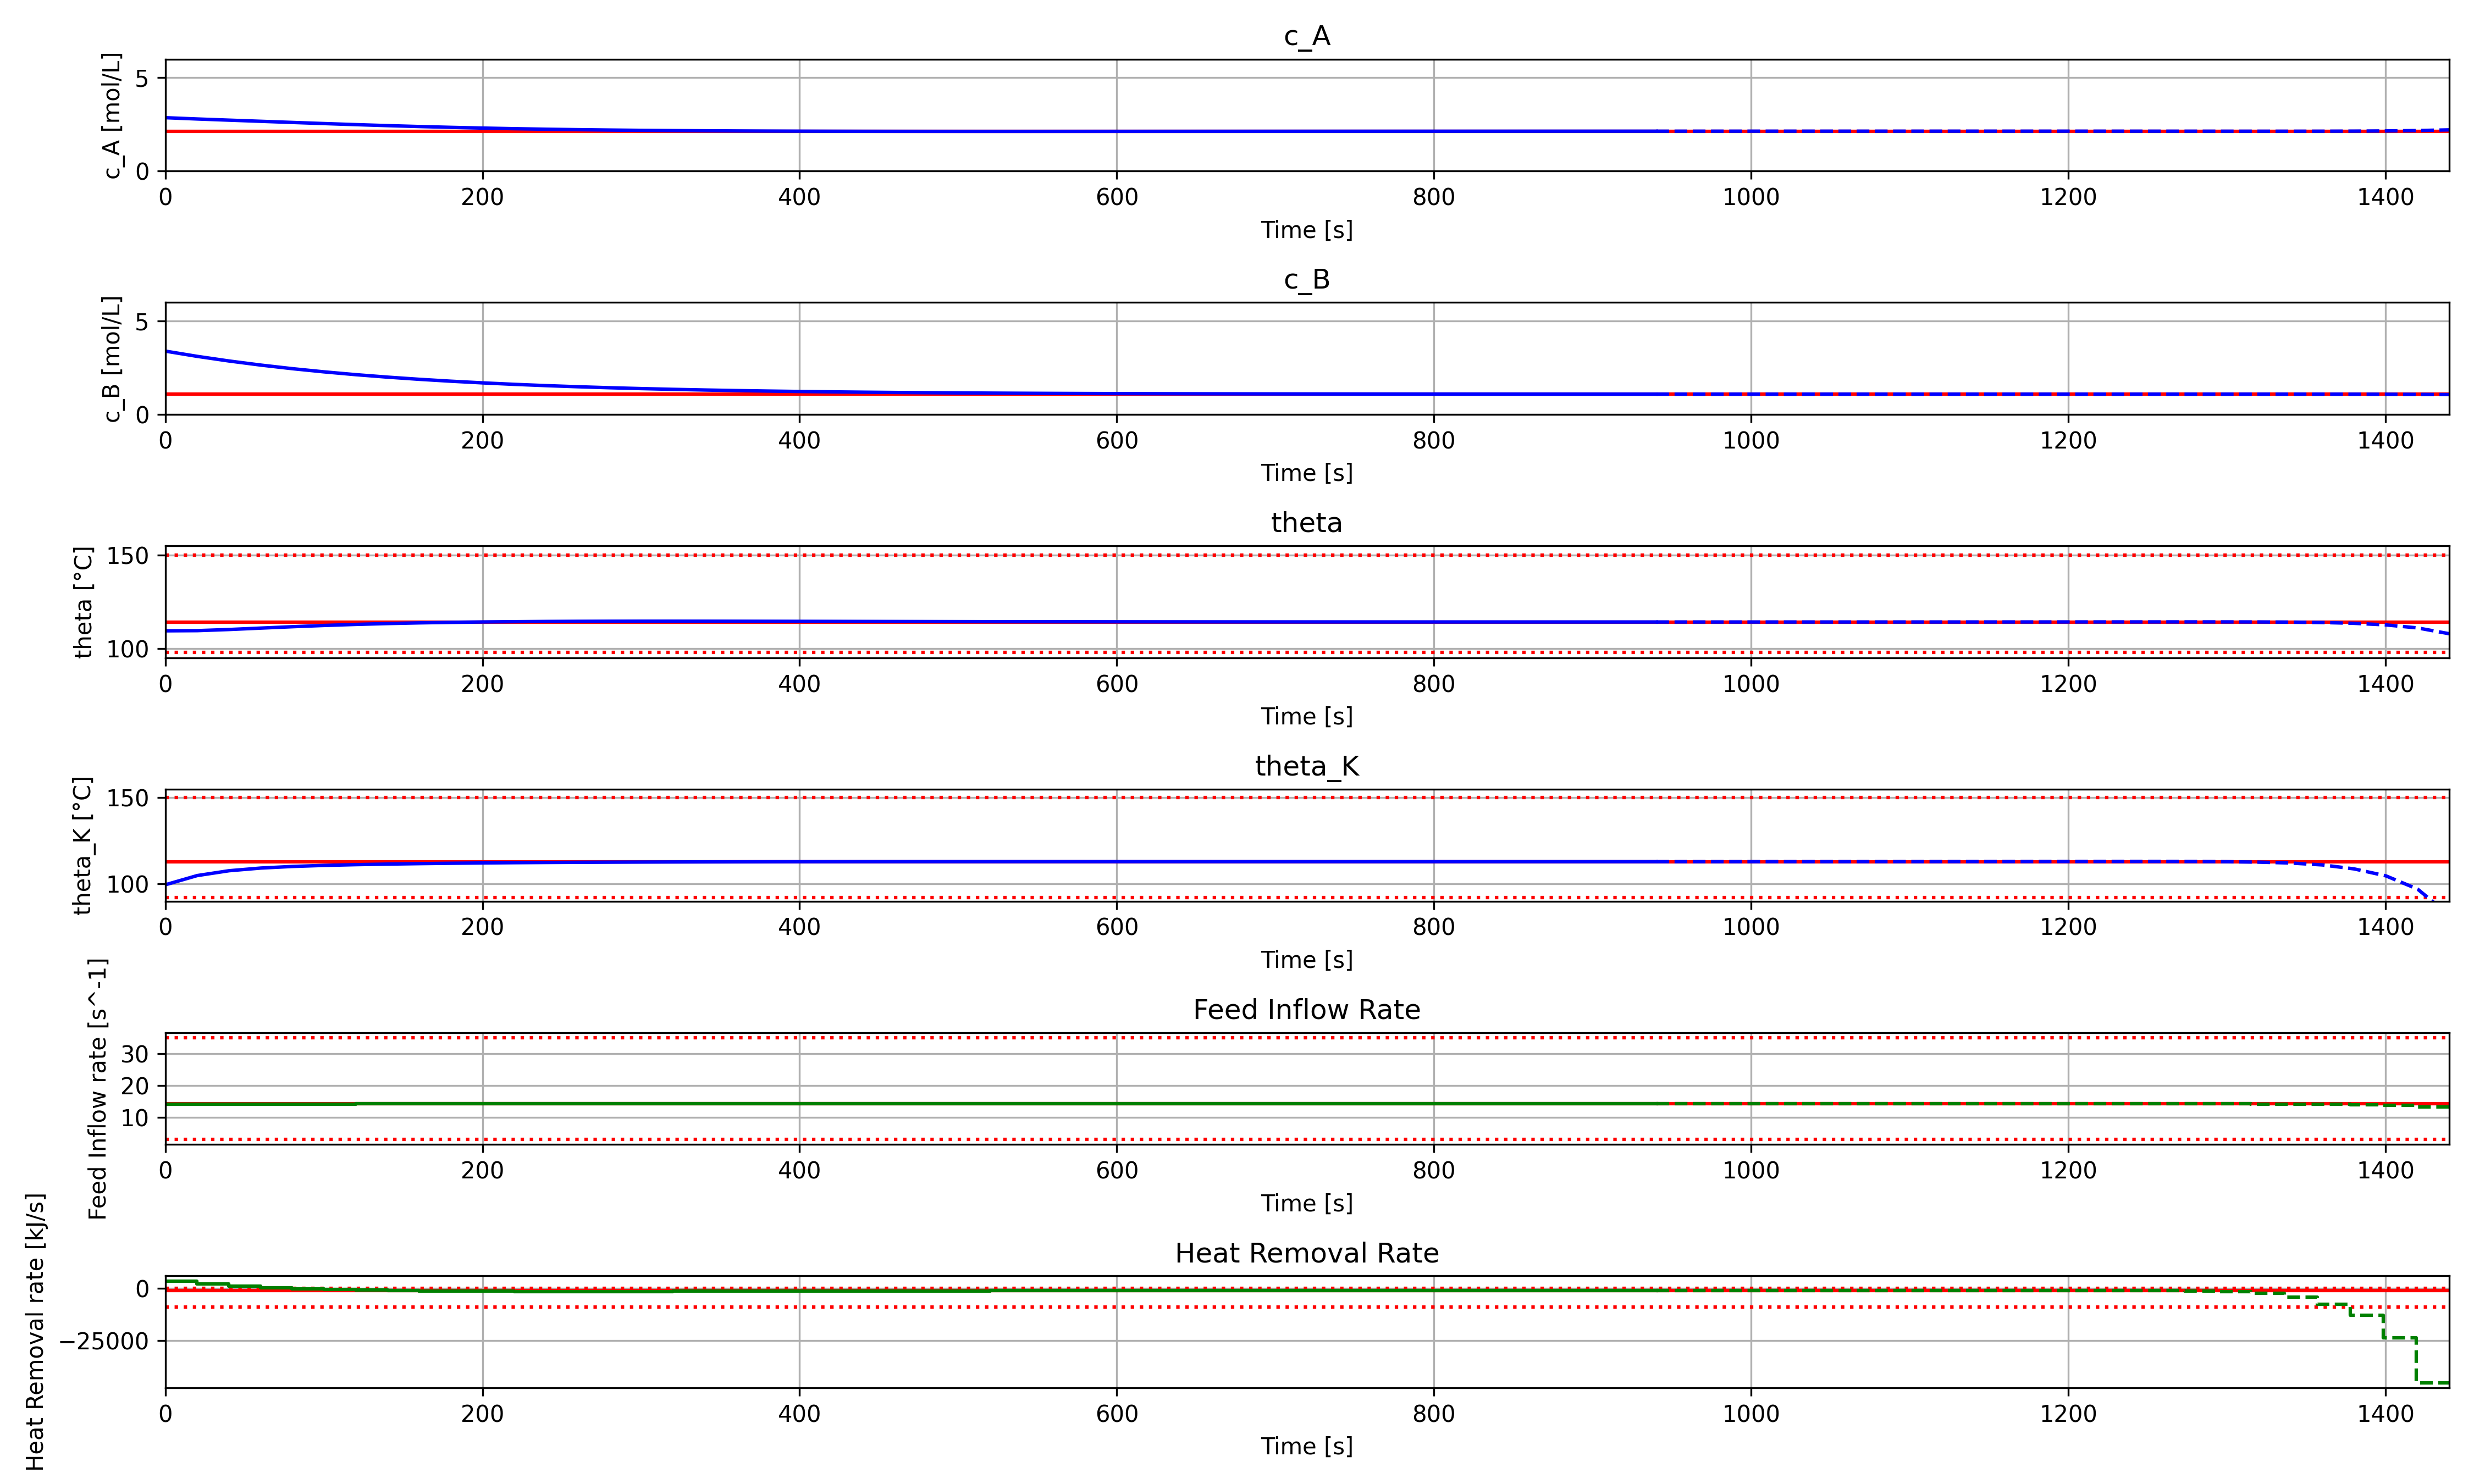
\includegraphics[width=15cm]{images/closedloop_traj_rrlb_1_1_25_not_converge.png}
			\caption{$\epsilon=1.0e-3$}
		\end{subfigure}
		\begin{subfigure}{15cm}
			\centering
			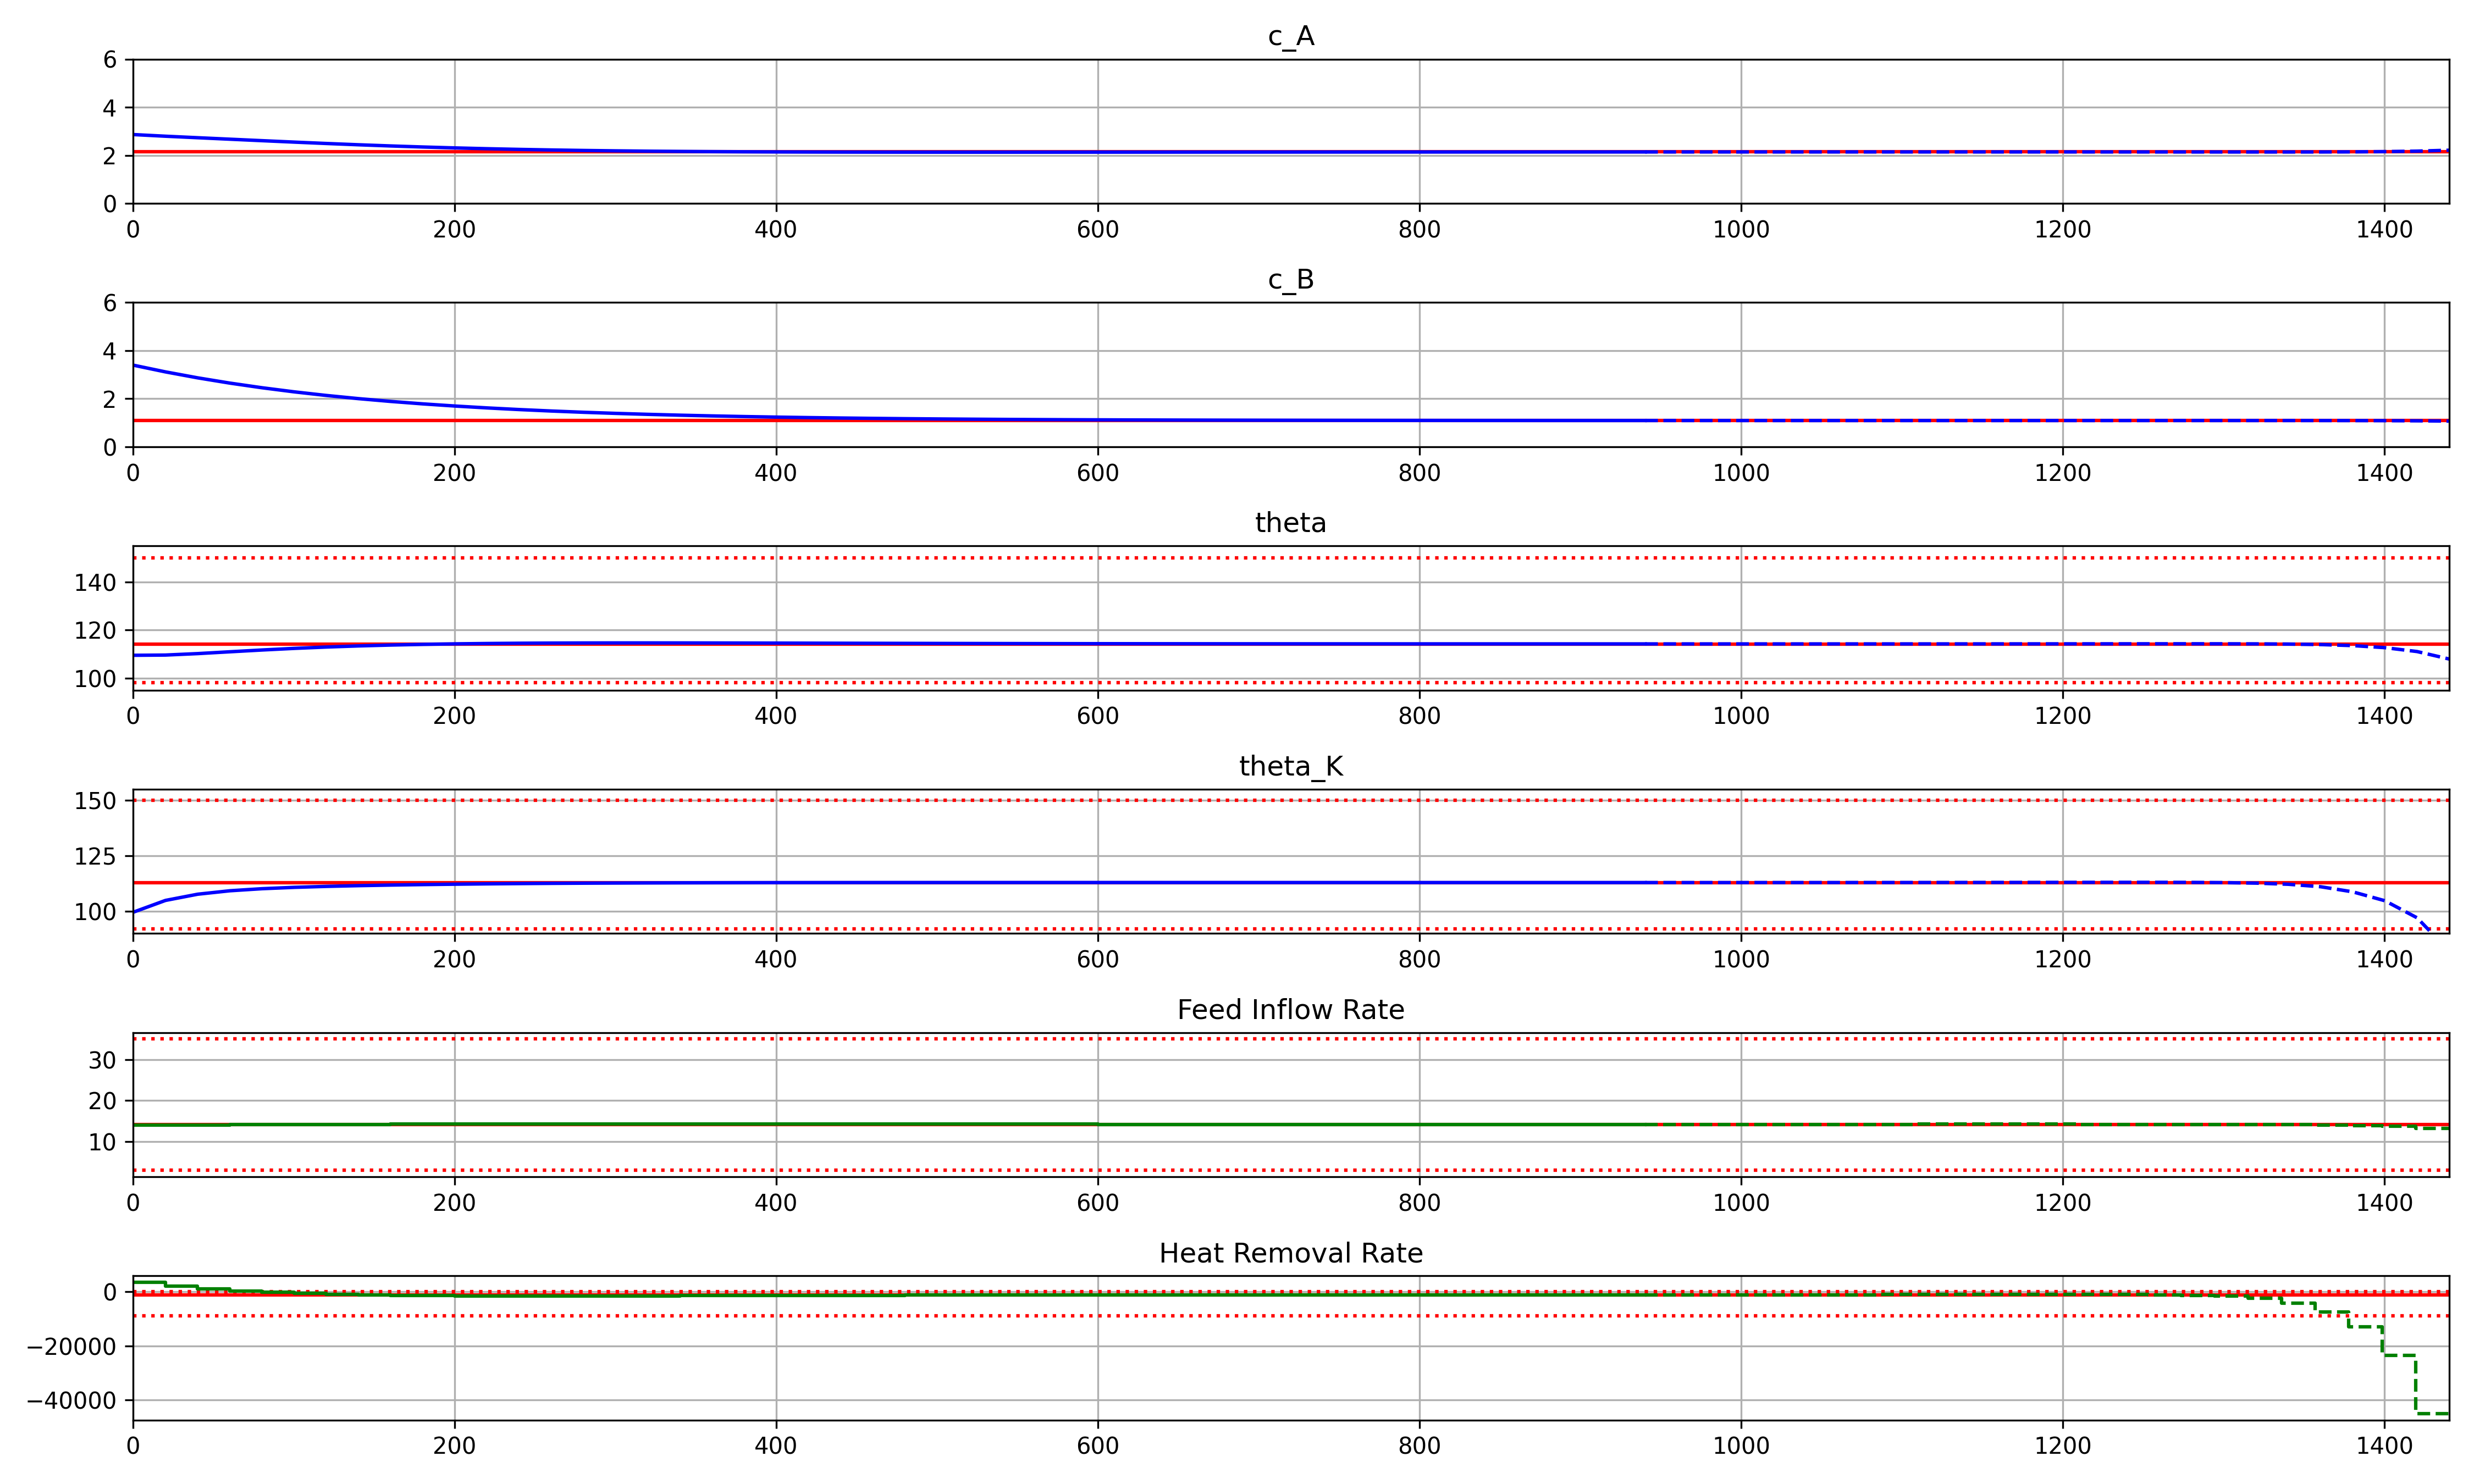
\includegraphics[width=15cm]{images/closedloop_traj_rrlb_1_1_25_converge.png}
			\caption{$\epsilon=1.0e-8$}
		\end{subfigure}
		\caption{Closed-loop trajectories for the RRLB MPC with initial state n°1, reference point n°1 and horizon size 25}
		\label{fig:closedloop_traj_rrlb_1_1_25}
	\end{figure}

	\item In every situation, whe the horizon size was 50, the RRLB MPC did not converge before the 350 iterations either, however we see in the results that the performance measure is much closer to the one achieved with horizon sizes 100 and 250 (when convergence was observed).
	This could indicate that the system actually stabilizes to the desired reference point, but just slower, and has not yet reached the desired tolerance at the 350th iteration.
	By inspecting the closed-loop trajectory in figure~\ref{fig:closedloop_traj_rrlb_1_1_50} we can see that this is indeed the case.
	The final (relative) discrepancy on the state is actually $6.71e-3$, which is quite close to the $1.0e-3$ tolerance.

	\begin{figure}[!ht]
		\centering
		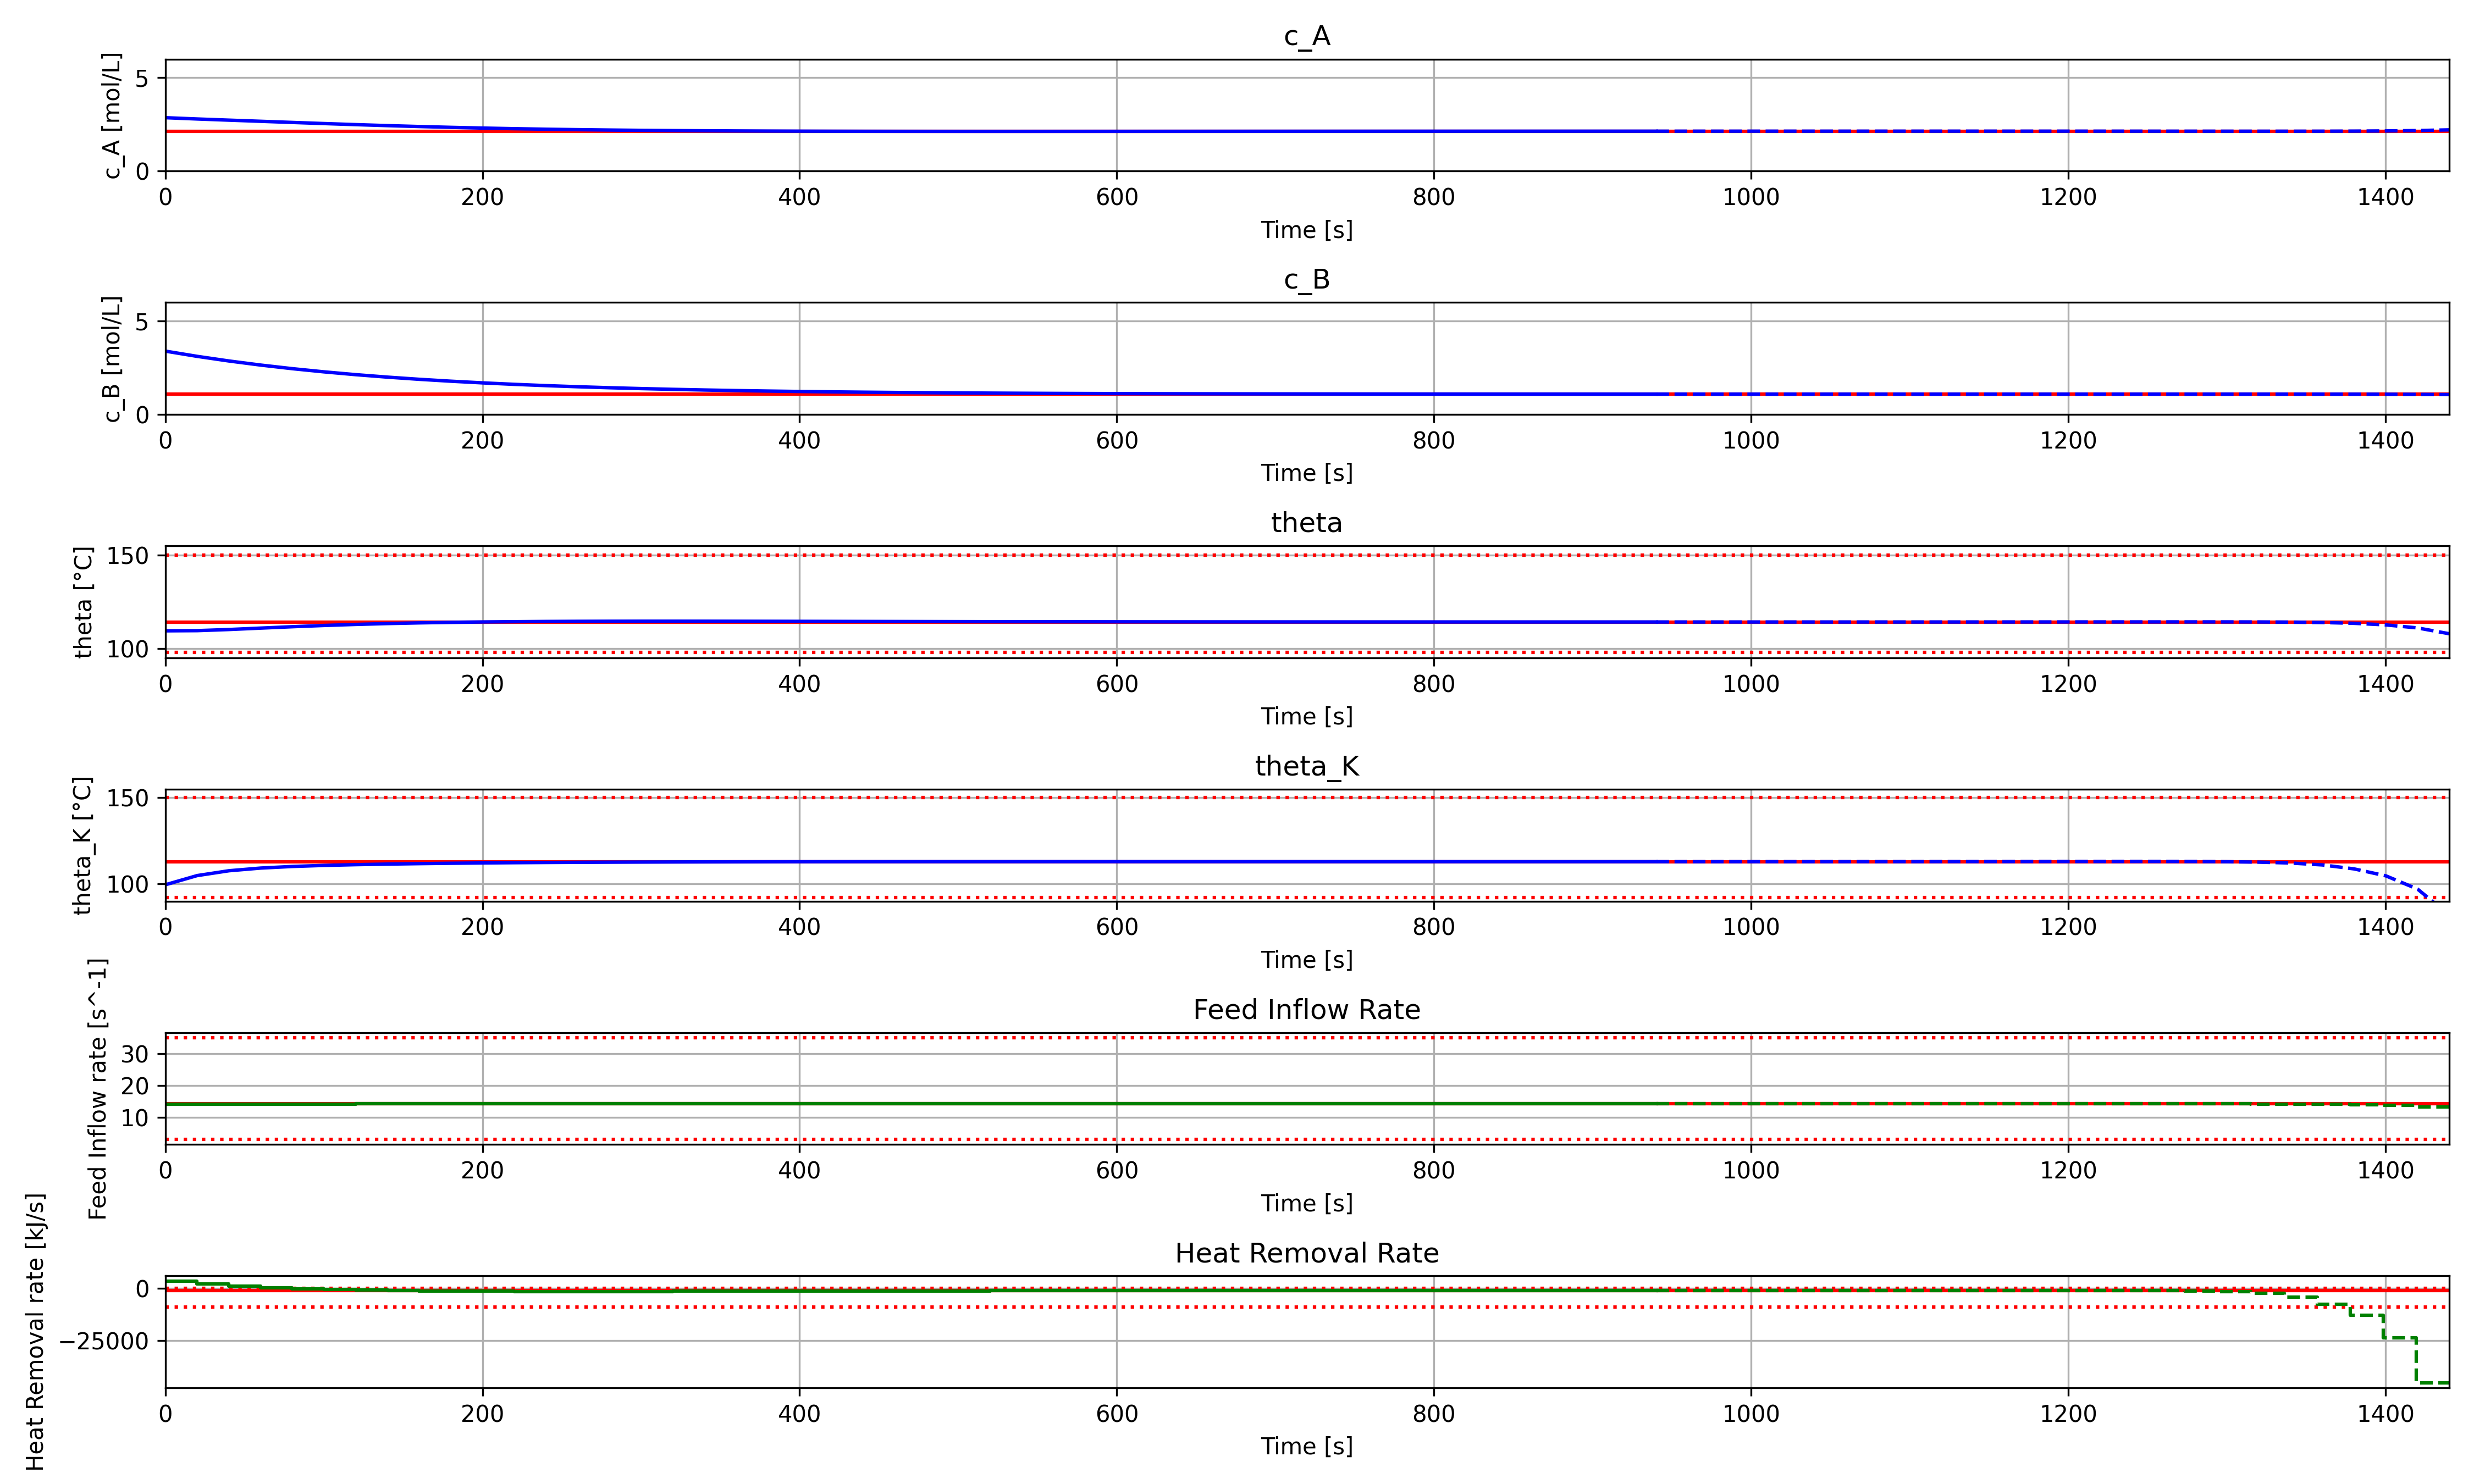
\includegraphics[width=15cm]{images/closedloop_traj_rrlb_1_1_50.png}
		\caption{Closed-loop trajectory for the RRLB MPC with initial state n°1, reference point n°1 and horizon size 50}
		\label{fig:closedloop_traj_rrlb_1_1_50}
	\end{figure}

	\item For horizon sizes 100 and 250, the RRLB MPC always converged to the desired objective and what ca be observed is that it always converged faster than regular MPC, in fewer iterations, and with smaller performance measure.
	In half of the situations this is caused by some constraint violation that allows the MPC to take "shortcuts", i.e. some trajectories that might be have a lower cost, but that are do not verify all the constraints.
	We used our script \verb|exp_analysis.py| to check case by case that this was indeed the case.
	In the other half, the improvements are quite substantial and their average (aggregated along the situations) can be found in figure~\ref{fig:improvement-percentages}.

	\begin{figure}[!ht]
		\centering
		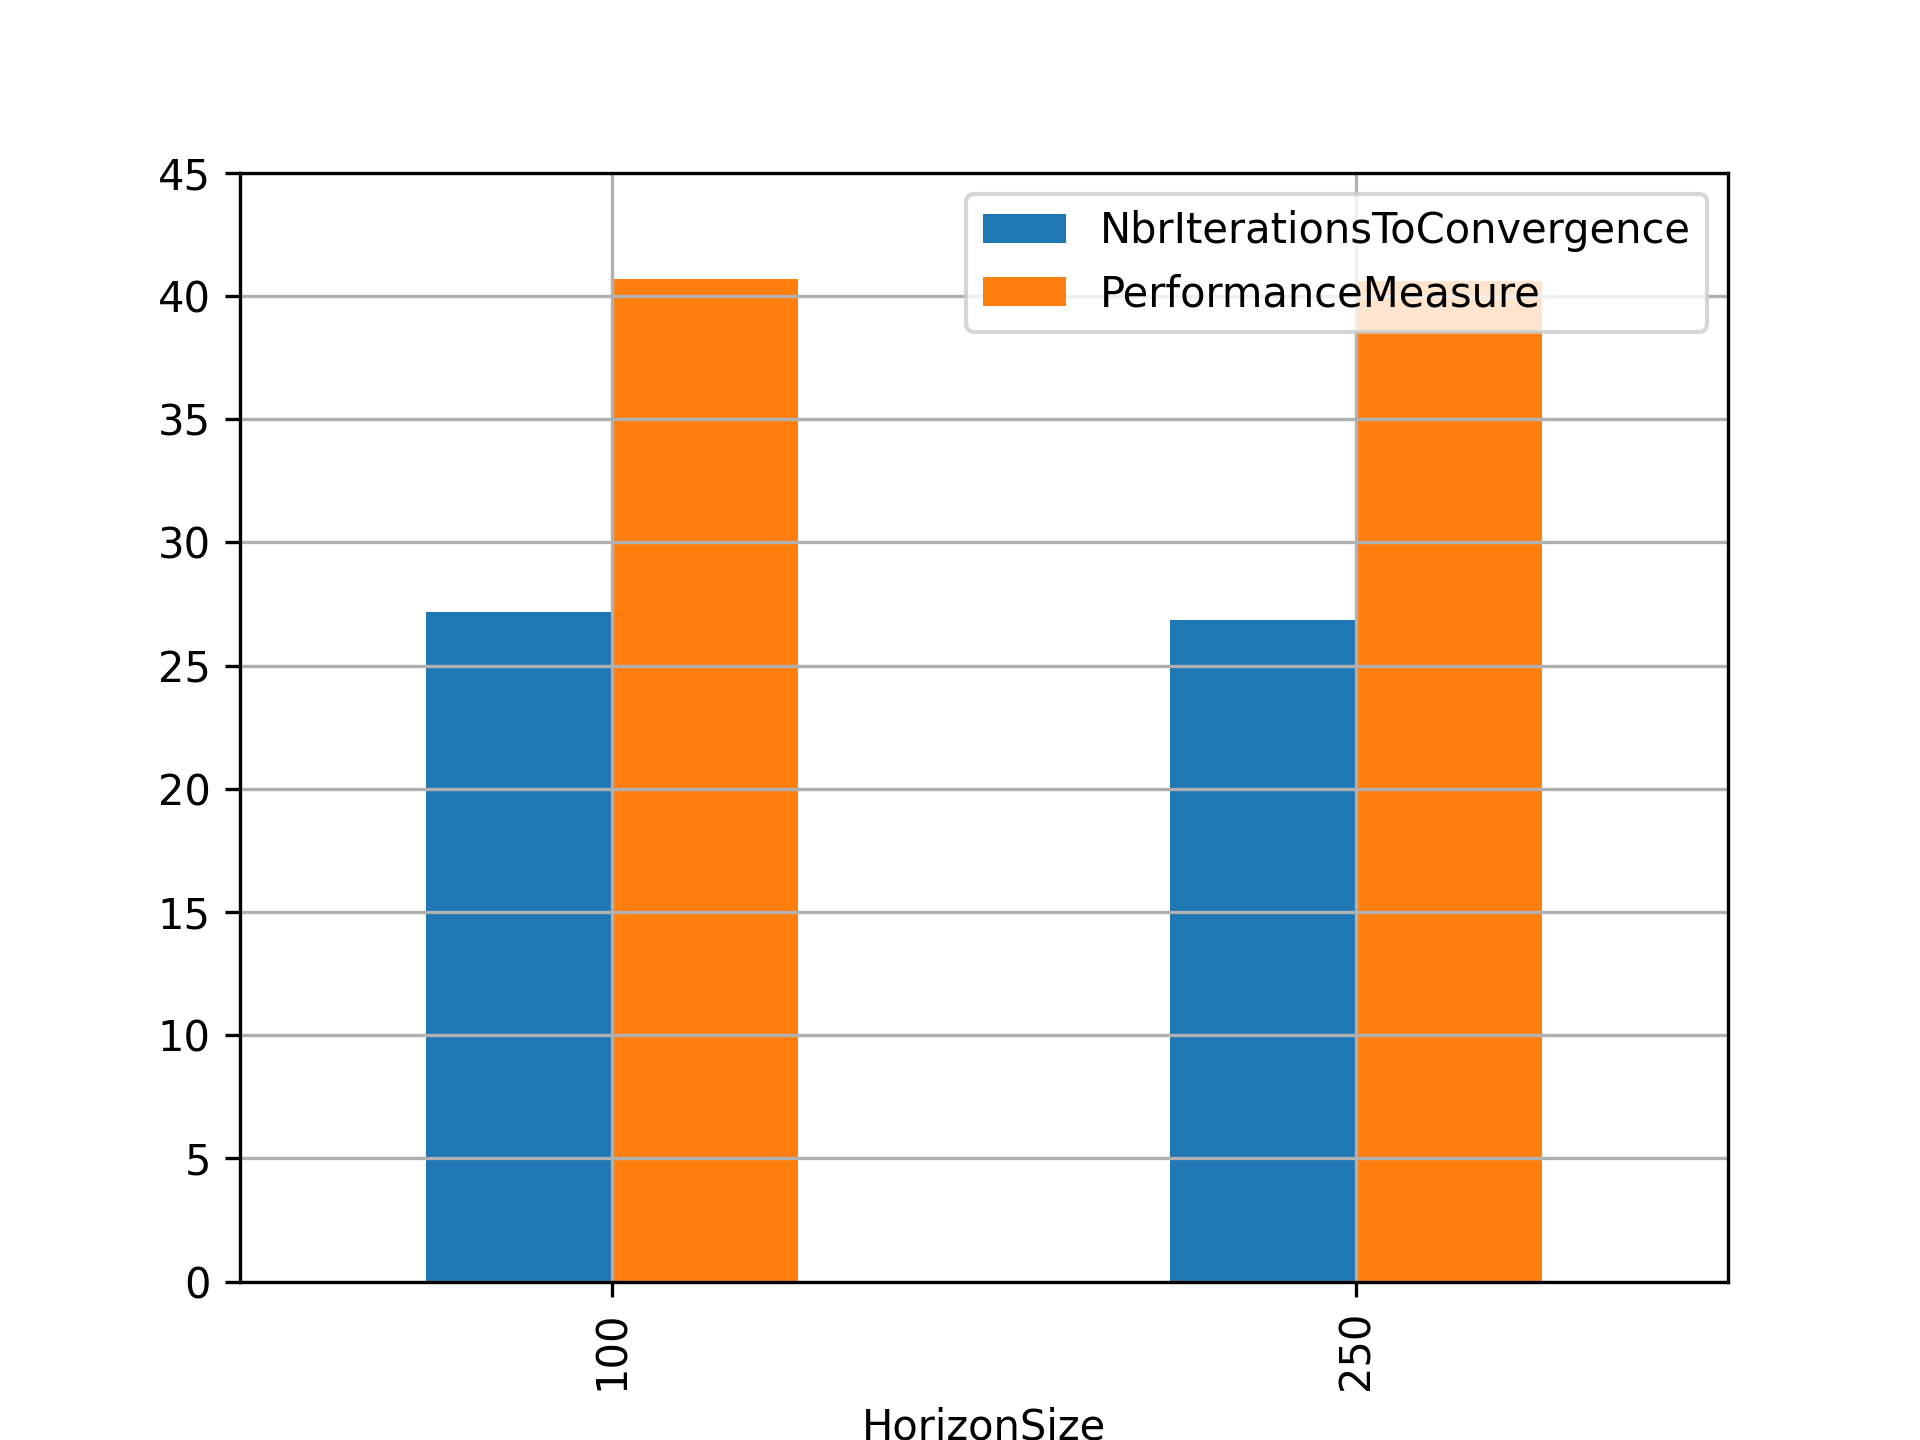
\includegraphics[width=7cm]{images/exp_all_improvement_percentages.png}
		\caption{Average improvement in percentage of the Number of iterations to convergence and the Performance measure of RRLB MPC compared to regular MPC}
		\label{fig:improvement-percentages}
	\end{figure}

	\item In general, we can see that augmenting the horizon size always improves the number of iterations needed to converge and the performance measure, for RRLB as for regular MPC.
	This general property of MPC is linked to the Bellman principle of optimality cited in~\ref{sec:what-is-MPC}, which suggests that the infinite horizon MPC is optimal, and that this optimum is better and better approximated as $N\to\infty$\,.

	\item The fact that the RRLB MPC only converges for a big enough horizon could be explained by the proof of theorem~\ref{thm:nominal-stability} in which the actual condition we needed to prove the descent property was that $\tilde{x}_N$ had to belong to the neighborhood given by the paragraph 2.5.5 of \cite{MPC-book}, let's call it $\calN_0$.
	Consequently, we could suppose the existence of a larger neighborhood $\calN_N$ such that $x\in\calN_N\implies \tilde{x}_N(x)\in\calN_1$, and imagine that $\calN_N$ gets monotonically larger as $N\to\infty$.
	Intuitively, this last property could be motivated by the fact that as the horizon size increases, the MPC has more time to reach $\calN_0$.
	However, these properties are out of the scope of this paper and could be the object of further research on the subject of RRLB MPC.

	\item As suggested by the figure~\ref{fig:runtimes}, RRLB seems i average a bit more computationally demanding.
	The main difference appears to be in the sensitivity computation time, which is understandable given their more complex form involving the gradients and hessians of RRLB functions shown in appendix~\ref{sec:osqp-condensation}.

	\begin{figure}[!ht]
		\centering
		\begin{subfigure}{.5\linewidth}
			\centering
			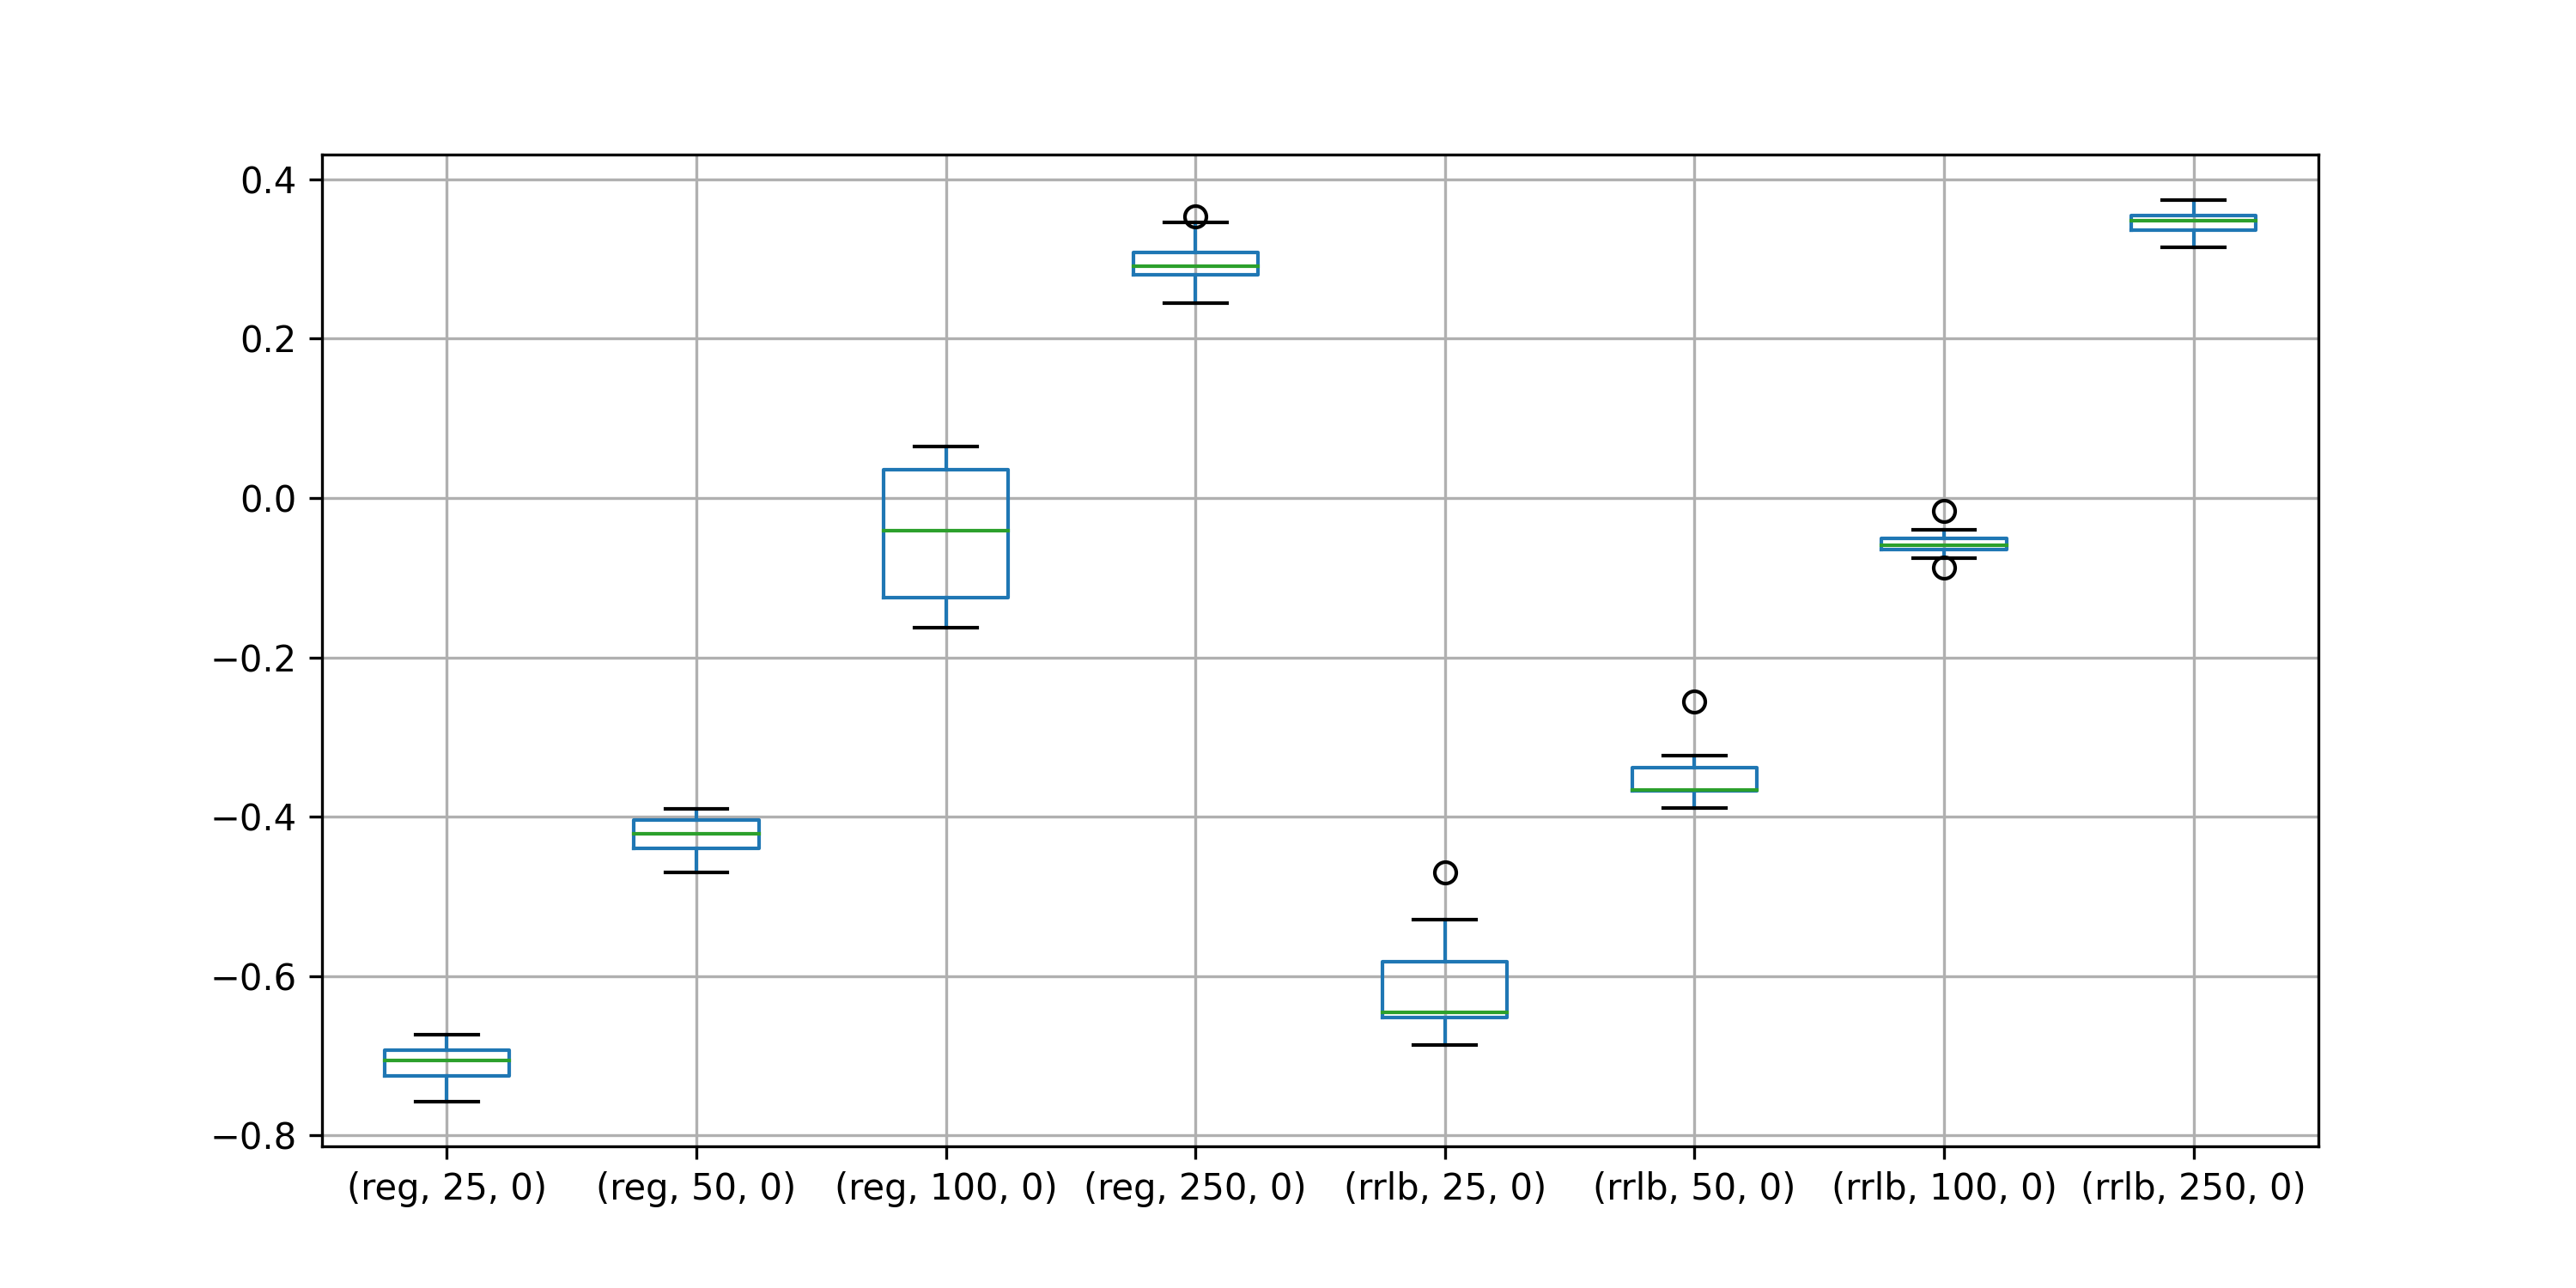
\includegraphics[width=1.0\textwidth]{images/exp_all_plot_runtimes_1.png}
			\caption{Average sensitivities computation times \\(in log scale) throughout the experiments}
			\label{fig:sensitivity-times}
		\end{subfigure}\,%
		\begin{subfigure}{.5\linewidth}
			\centering
			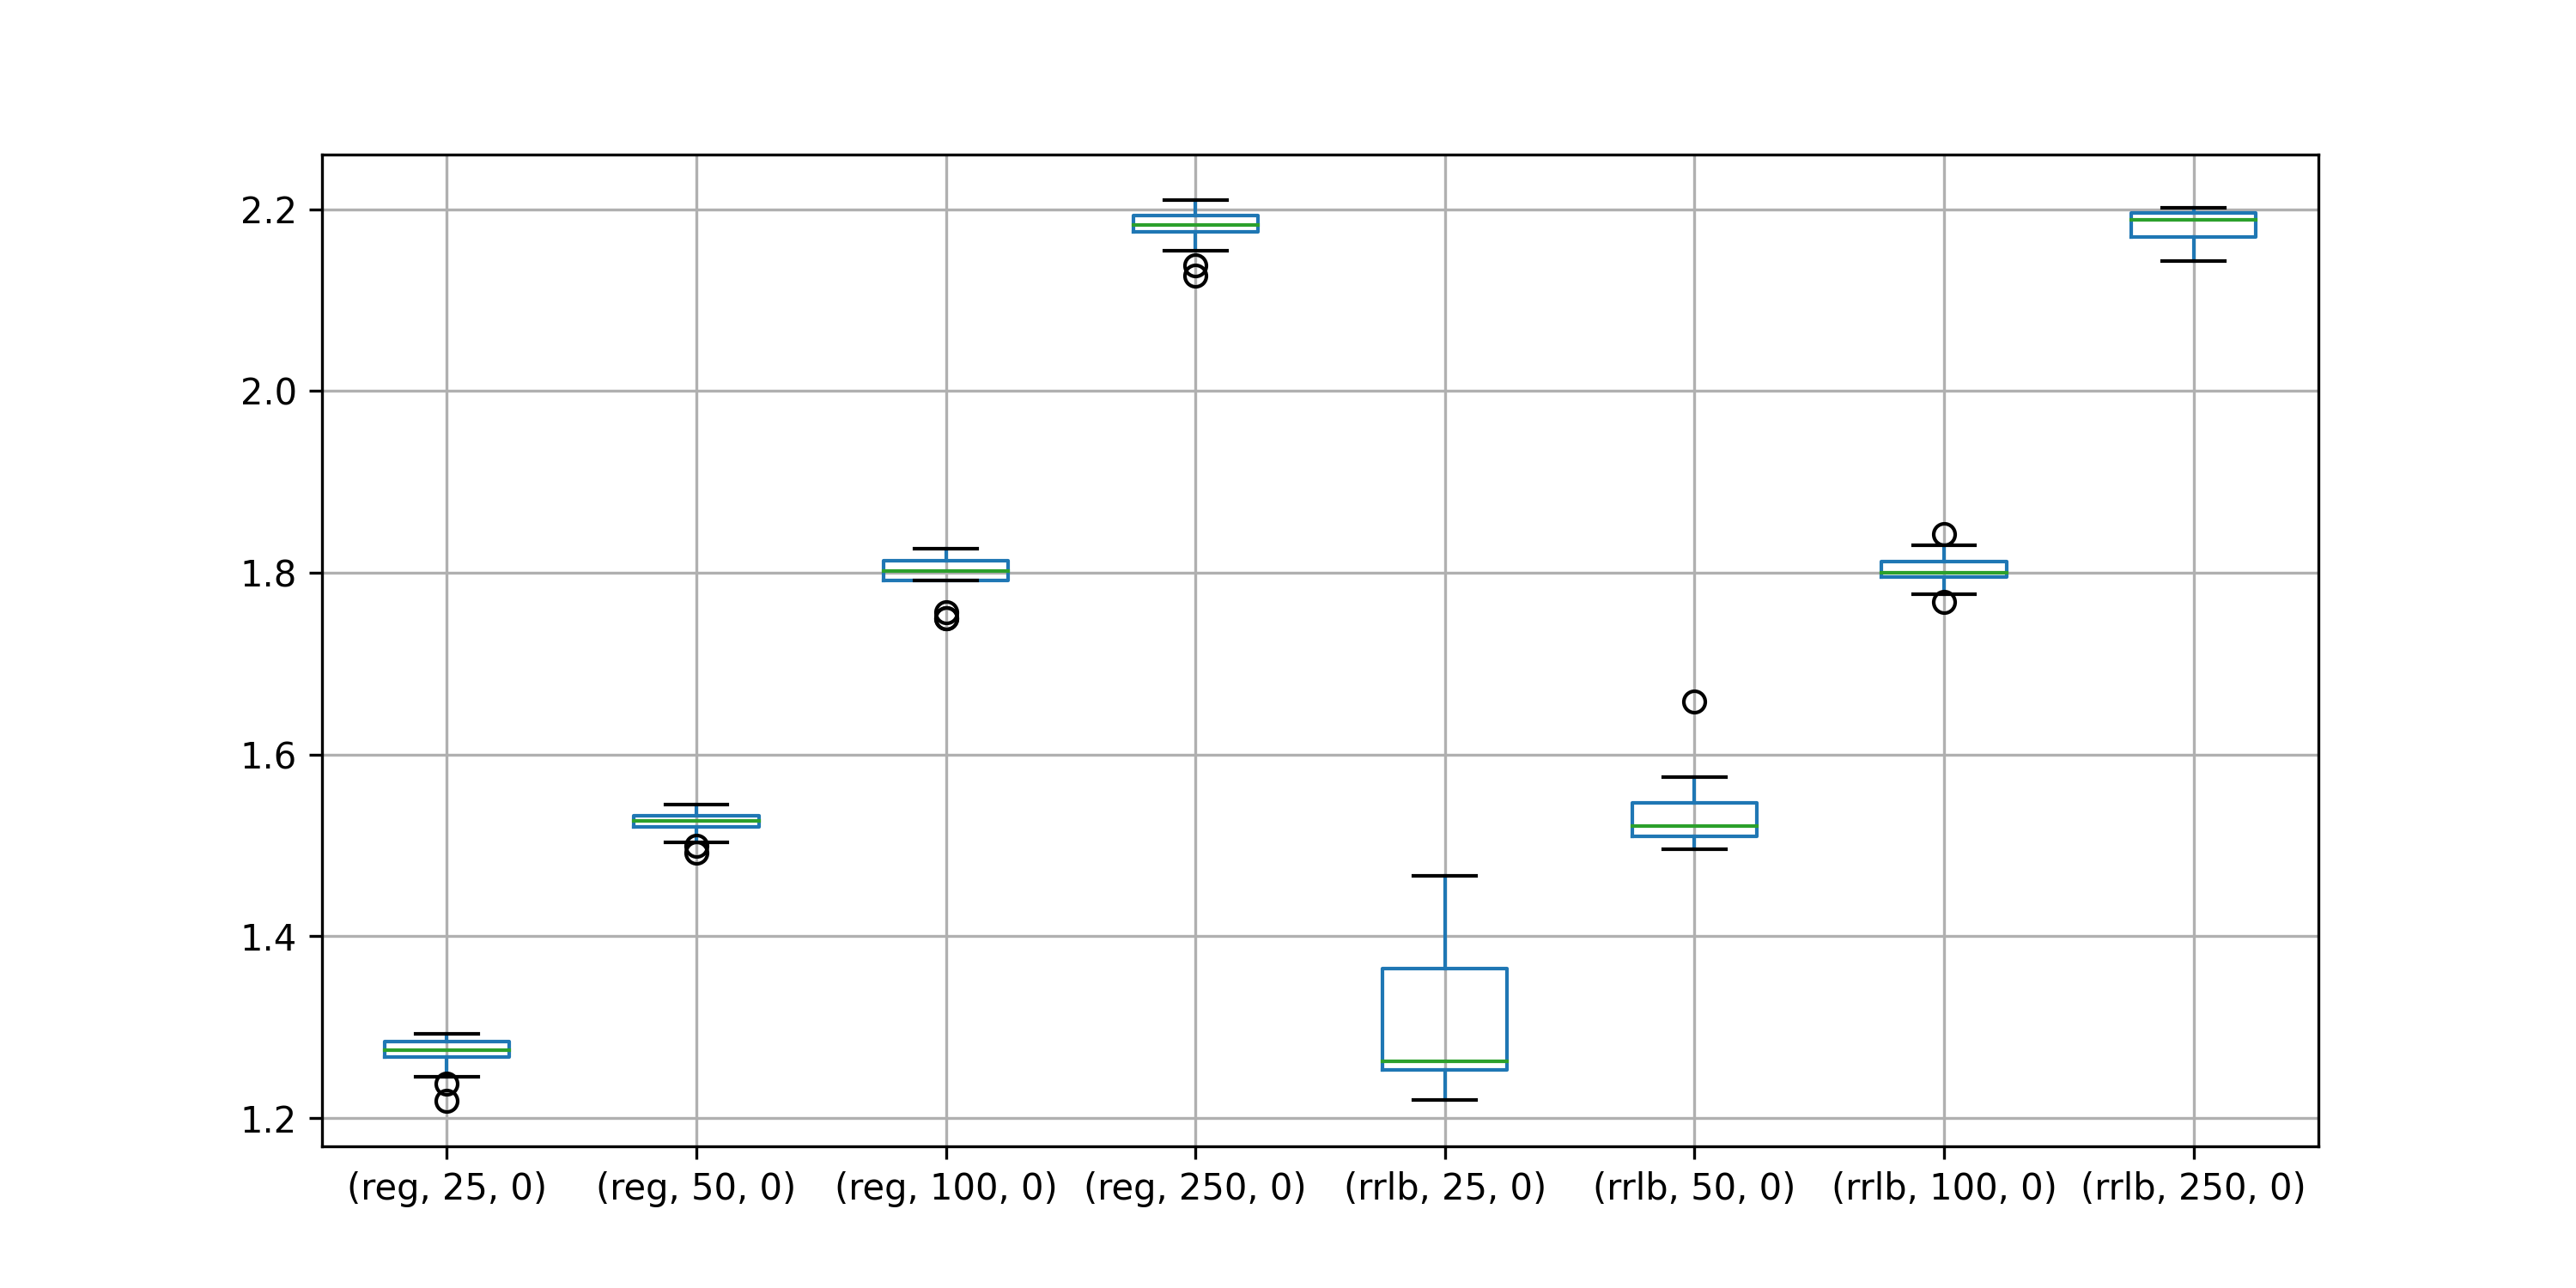
\includegraphics[width=1.0\textwidth]{images/exp_all_plot_runtimes_2.png}
			\caption{Average condensation times (in log \\ scale) throughout the experiments}
			\label{fig:condensation-times}
		\end{subfigure}\newline
		\begin{subfigure}{.5\linewidth}
			\centering
			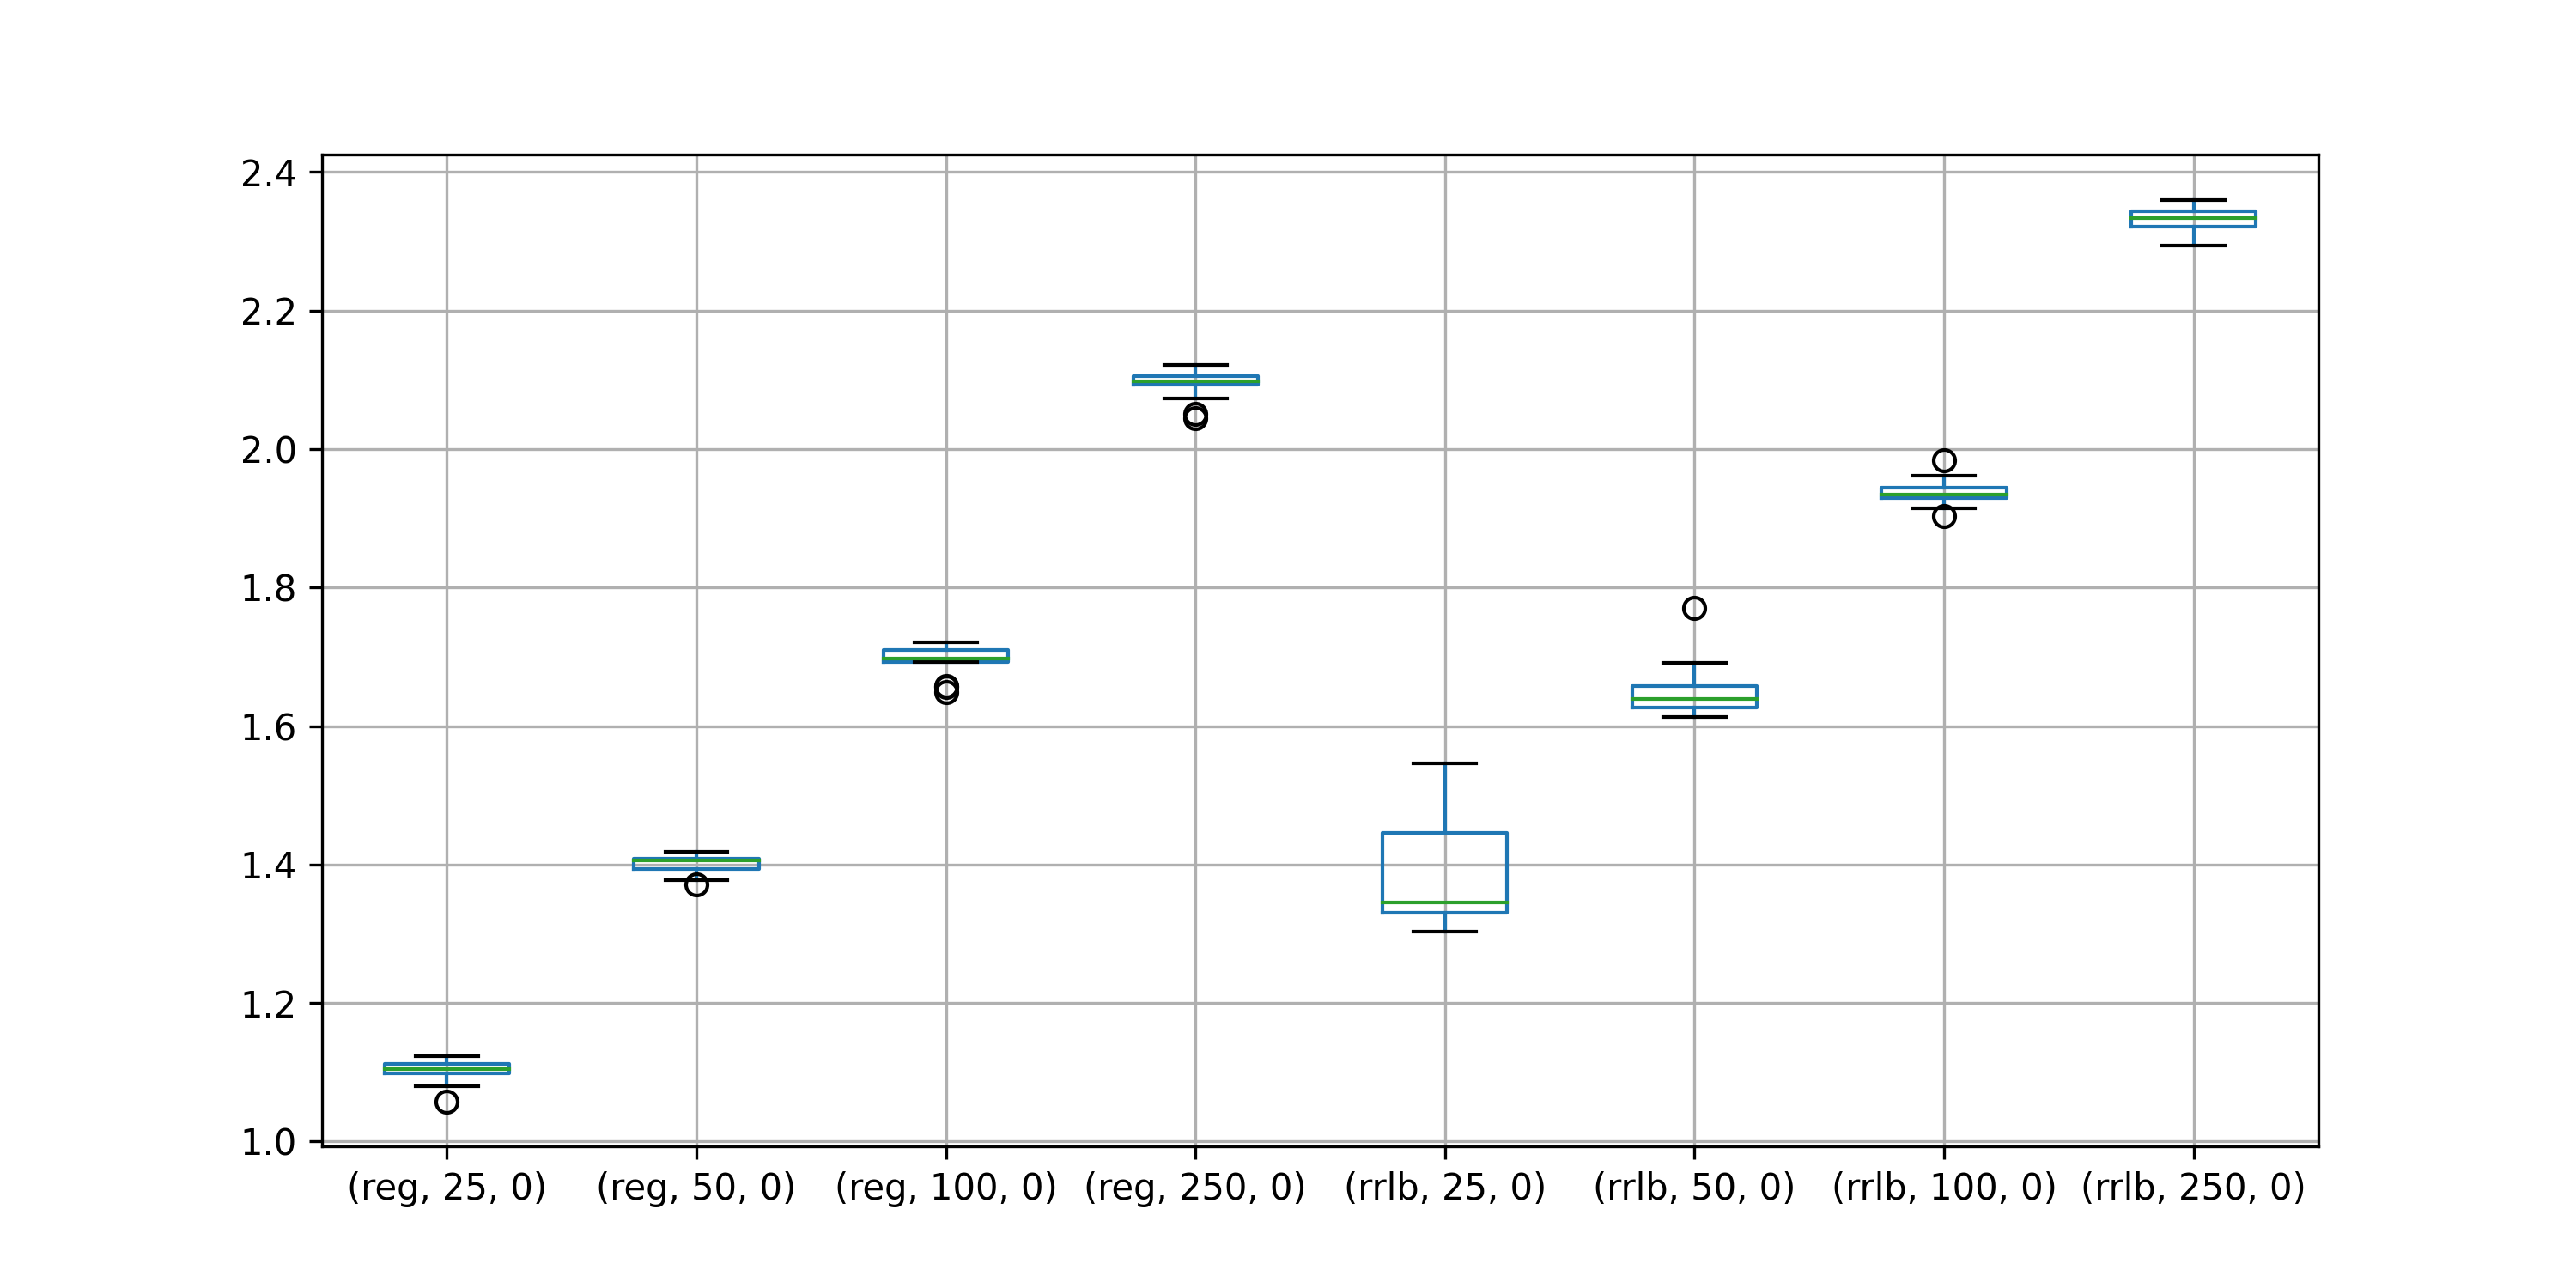
\includegraphics[width=1.0\textwidth]{images/exp_all_plot_runtimes_3.png}
			\caption{Average solving times (in log scale) throughout the experiments}
			\label{fig:solving-times}
		\end{subfigure}

		\caption{Boxplots of runtimes for different phases of RTI, averaged by scheme and horizon length}
		\label{fig:runtimes}
	\end{figure}

\end{itemize}

\section{Conclusion and outlook}

Throughout this report, we have explored the theory of MPC and RRLB MPC, and we have managed to show two remarkable results.
Nevertheless, several questions on the subject remain open.
Here is a non-exhaustive list of the ones that came up during the semester:
\begin{itemize}[label=\textbullet]
	\item How do the parameters $\epsilon$ and $\delta$ really influence the behavior of the scheme ? In particular, are there ways to determine values for those parameters that always ensure asymptotic stability and/or constraint satisfaction ?
	% These questions are not trivial since our current work does not give enough insight on the

	\item Could we improve our numerical results by using 2 or more iterations of SQP in our RTI scheme ?

	\item If we move the initial state away from the reference point, will the regular MPC scheme yield divergent trajectories before RRLB MPC (for suitable horizon lengths) ?

	\item Could we improve the description of the neighborhood provided by theorem~\ref{thm:nominal-stability} by proving the kind of monotonicity property evoked in section~\ref{sec:results-discussion} ?
\end{itemize}


\newpage

\section{Appendix}

\subsection{Controllable vs. Stabilizable}\label{sec:controllability-stabilizability}

The notions of controllability and stabilizability are central in control theory and are the first hypothesis one should plan to verify on a concrete system.
They are intrinsic properties of the equation describing the evolution of the system (either an ODE for a continuous-time system or a map for a discrete-time system) and could roughly be defined as follows:
\begin{itemize}[label=\textbullet]
	\item A system is \textit{controllable} if it can be steered from any feasible state to any other reference state in a finite time.
	\item A system is \textit{stabilizable} if it can be steered from any feasible state to any other feasible state in an infinite time, or equivalently that it asymptotically approaches this reference state.
\end{itemize}

These definitions can be made formal in the case of linear time invariant (or LTI) dynamics of the form $\dot{x}=Ax+Bu$ in the continuous-time case, and $x^+=Ax+Bu$ in the discrete-time case:
\begin{definition}[Controllability]~
	\begin{itemize}[label=\textbullet]
		\item A continuous LTI dynamical system $\dot{x}=Ax+Bu$ is controllable if $\forall\lambda\in\rm{eig}(A),~\rank(A-\lambda I_{n_x},B)=n_x$ or equivalently if
		$$\rank\underbrace{\begin{pmatrix}B&\vline& AB&\vline&\ldots&\vline&A^{n_x-1}B\end{pmatrix}}_{:=C}=n_x$$
		where $C$ is called the \textit{controllability matrix}.

		\item A discrete LTI system $x^+=Ax+Bu$ is controllable if any of the conditions above holds for $(A,B)$.
	\end{itemize}
\end{definition}
\begin{definition}[Stabilizability]~
	\begin{itemize}[label=\textbullet]
		\item A continuous LTI dynamical system $\dot{x}=Ax+Bu$ is stabilizable if $\forall\lambda\in\R,~\rank(A-\lambda I_{n_x},B)\leq n_x\implies \Re(\lambda)< 0$ or equivalently if $\exists K\in\R^{n_x\times n_u}~:~A+BK$ is Hurwitz, i.e. only has eigenvalues with negative real part.

		\item A discrete LTI system $x^+=Ax+Bu$ is stabilizable if any of the conditions above holds for $(A,B)$.
	\end{itemize}
\end{definition}

\begin{remark}
	The stabilizable matrix $K$ can be explicitly constructed in the case of LQR as mentioned in section~\ref{sec:what-is-MPC}.
\end{remark}

\subsection{Derivation of the classical DARE}\label{sec:DARE}

If we consider the LQR problem presented in~\ref{sec:what-is-MPC}, then Bellman's principle of optimality reads:

$$V_\infty(x)=\min_{u\in\R^{n_u}}~\underbrace{x^TQx+u^TRu+V_\infty(Ax+Bu)}_{=:\phi(x,u)}$$

If we suppose that $V_\infty$ is itself a quadratic function, i.e. $V_\infty(x)=x^TPx$, then the first order optimality conditions at a minimizer $u^*$ are:
$$\nabla_u\phi(x,u^*)=2Ru^*+2B^TP(Ax+Bu^*)=0\implies u^*=\underbrace{-\inv{R+B^TPB}B^TPA}_{=:K}x$$
and by plugging this value back into the minimization problem and developing the form of $K$, we can obtain the DARE:
\begin{align*}
	V_\infty(x)=x^TPx&=x^TQx+u^{*~T}Ru^*+V_\infty(Ax+Bu^*)\\
	&=x^TPx=x^TQx +x^TK^TRKx+V_\infty((A+BK)x)\\
	&=\cdots=x^T(Q+A^TPA-A^TPB(R+B^TPB)^{-1}B^TPA)x\\
	\implies&\boxed{P=Q+A^TPA-A^TPB(R+B^TPB)^{-1}B^TPA}
\end{align*}


\subsection{OSQP condensation}\label{sec:osqp-condensation}

If we consider the optimization variable of the QP subproblem (as described in section~\ref{sec:RTI-scheme}) to be $z=(\Delta x_0,\ldots,\Delta x_N,\Delta u_0, \ldots,\Delta u_{N-1})$, and we write $x$ for the system's current state and  $(x_0^{init},\ldots,x_{N}^{init},u_0^{init},\ldots,u_{N-1}^{init})$ for the initial guess (obtained by shift), then the matrices and vectors in the OSQP formulation will be:
\scriptsize
\begin{align*}
	q_{OSQP}&=2\begin{pmatrix}
		Q&&&&&&\\
		&\ddots&&&&&\\
		&&Q&&&&\\
		&&&P&&&\\
		&&&&R&&\\
		&&&&&\ddots&\\
		&&&&&&R
	\end{pmatrix}\begin{pmatrix}
		x_0^{init}\\\vdots\\x_N^{init}\\u_0^{init}\\\vdots\\u_{N-1}^{init}
	\end{pmatrix}+\color{blue}\epsilon\begin{pmatrix}
		\nabla B_x(x_0^{init})\\\vdots\\\nabla 0\\\nabla B_u(u_0^{init})\\\vdots\\\nabla B_u(u_{N-1}^{init})
	\end{pmatrix}\color{black}\\
	P_{OSQP}&=4\begin{pmatrix}
		Q&&&&&&\\
		&\ddots&&&&&\\
		&&Q&&&&\\
		&&&P&&&\\
		&&&&R&&\\
		&&&&&\ddots&\\
		&&&&&&R
	\end{pmatrix}+\color{blue}2\epsilon\begin{pmatrix}
		\nabla^2B_x(x_0^{init})&&&&&\\
		&\ddots&&&&\\
		&&0&&&\\
		&&&\nabla^2B_u(u_0^{init})&&\\
		&&&&\ddots&\\
		&&&&&\nabla^2B_u(u_{N-1}^{init})
	\end{pmatrix}\color{black}
\end{align*}

$$A_{OSQP}=\begin{pmatrix}
	I_{n_x}&&&&&0&&&&\\
	A_{0}^{init}&-I_{n_x}&&&&B_{0}^{init}&\ddots&&\\
	&A_{1}^{init}&-I_{n_x}&&&&\ddots&&\\
	&&\ddots&\ddots&&&&&\\
	&&&A_{N-1}^{init}&-I_{n_x}&&&B_{N-1}^{init}&0\\
	\color{red}C_x&&&&&&&&\\
	&\color{red}C_x&&&&&&&\\
	&&\color{red}\ddots&&&&&&\\
	&&&\color{red}C_x&&&&&\\
	&&&&\color{red}C_x&&&&\\
	&&&&&\color{red}C_u&&&\\
	&&&&&&\color{red}\ddots&&\\
	&&&&&&&\color{red}\ddots&\\
	&&&&&&&&\color{red}C_u
\end{pmatrix}$$

$$l_{OSQP}=\begin{pmatrix}
	x-x_0^{init}\\x_{1}^{init}-f(x_0^{init},u_0^{init})\\\vdots\\x_{N}^{init}-f(x_{N-1}^{init},u_{N-1}^{init})\\\color{red}-\infty\\\color{red}\vdots\\\color{red}-\infty
\end{pmatrix}\qquad u_{OSQP}=\begin{pmatrix}
	x-x_0^{init}\\x_{1}^{init}-f(x_0^{init},u_0^{init})\\\vdots\\x_{N}^{init}-f(x_{N-1}^{init},u_{N-1}^{init})\\\color{red}d_x-C_xx_0^{init}\\\color{red}\vdots\\\color{red}d_x-C_xx_N^{init}\\\color{red}\vdots\\\color{red}d_u-C_uu_{0}^{init}\\\color{red}\vdots\\\color{red}d_u-C_uu_{N-1}^{init}
\end{pmatrix}$$
\normalsize
In the above, all the red terms only appear for regular MPC, and the blue terms only for RRLB MPC.

\subsection{CSTR model, constraints and MPC costs}\label{sec:cstr-model}
\noindent The evolution of the system is described by the following system of ODEs:
\begin{align*}
	\dot{c}_A(t)&=u_1(t)(c_{A0}-c_A(t))-k_1(\vartheta(t))c_A(t)-k_3(\vartheta(t))c_A(t)^2\\
	\dot{c}_B(t)&=-u_1(t)c_B(t)+k_1(\vartheta(t))c_A(t)-k_2(\vartheta(t))c_B(t)\\
	\dot{\vartheta}(t)&=u_1(t)(\vartheta_0-\vartheta(t))+\frac{k_wA_R}{\rho C_pV_R}(\vartheta_K(t)-\vartheta(t))\\
	&\qquad-\frac{1}{\rho C_p}\left[ k_1(\vartheta(t))c_A(t)H_1+k_2(\vartheta(t))c_B(t)H_2 +k_3(\vartheta(t))c_A(t)^2H_3\right]\\
	\dot{\vartheta}_K(t)&=\frac{1}{m_KC_{PK}}\left[ u_2(t)+k_wA_R(\vartheta(t)-\vartheta_K(t)) \right]
\end{align*}
where $k_i(\vartheta)=k_{i,0}\exp\left(\frac{E_i}{\vartheta+273.15}\right)$ for $i=1,2,3$\,.
All the coefficients appearing in these equations are given in table~\ref{tab:cstr-model-coefficients}:
\begin{table}[H]
	\centering
	\begin{tabular}{|c|c||c|c|}
		\hline
		Symbol&Value&Symbol&Value\\
		\hline
		$k_{10}$ & $1.287e12\,h^{-1}$ & $\rho$ & $0.9342\,\frac{kg}{L}$\\
		$k_{20}$ & $1.287e12\,h^{-1}$ & $C_p$ & $3.01\,\frac{kJ}{kg\cdot K}$\\
		$k_{30}$ & $9.043e9\,h^{-1}$ & $k_w$ & $4032\,\frac{kJ}{h\cdot m^2\cdot K}$\\
		$E_{1}$ & $-9758.3$ & $A_R$ & $0.215\,m^2$\\
		$E_{2}$ & $-9758.3$ & $V_R$ & $10\,L$\\
		$E_{3}$ & $-8560$ & $m_K$ & $5\,kg$\\
		$H_{1}$ & $4.2\,\frac{kJ}{mol}$ & $C_{PK}$ & $2.0\,\frac{kJ}{kg\cdot mol}$\\
		$H_{2}$ & $-11.0\,\frac{kJ}{mol}$ & $c_{A0}$ & $5.1\,\frac{mol}{L}$\\
		$H_{3}$ & $-41.85\,\frac{kJ}{mol}$ & $\vartheta_0$ & $104.9\,^\circ C$\\
		\hline
	\end{tabular}
	\caption{CSTR model coefficients}
	\label{tab:cstr-model-coefficients}
\end{table}

\noindent The constraints on the controls are given by the following equations:
\begin{align*}
	3.0\,h^{-1}\leq &~u_1~ \leq 25.0\,h^{-1}\\
	-9000.0\,\frac{kJ}{h}\leq &~u_2~ \leq 0.0\,\frac{kJ}{h}\\
\end{align*}
There were no constraints originally in \cite{diehl-dissertation}, but some were introduced in \cite{cstr-ref} on $\vartheta,\vartheta_K$.
We added some more to make sure that the feasible set of the states was polytopic and not just polyhedral (i.e. it is bounded), which ensures that the RRLB function exists.
\begin{align*}
	0.0\leq&~c_A~\leq 10.0\\
	0.0\leq&~c_B~\leq 10.0\\
	98.0\leq &~\vartheta~\leq 150.0\\
	92.0\leq &~\vartheta_K~\leq 150.0
\end{align*}

\noindent The costs are finally given by

$$Q=\begin{pmatrix}
	0.2\,mol^{-2}L^2 & 0 & 0 & 0\\
	0 & 1.0\,mol^{-2}L^2 & 0 & 0\\
	0 & 0 & 0.5^\circ C^{-2} & 0\\
	0 & 0 & 0 & 0.2^\circ C^{-2}
\end{pmatrix},\qquad R=\begin{pmatrix}
	0.5\,h^{2} & 0\\
	0 & 5.0e-7\,kJ^{-2}h^2
\end{pmatrix}$$

\newpage

\section{Bibliography}

\printbibliography


\end{document}
